% Turabian Formatting for Theses and Dissertations, 2018/08/06
%
% Developed using the turabian-formatting package (2018/08/01), available through CTAN: http://www.ctan.org/pkg/turabian-formatting
%
% Additional document class formatting options:
%
% raggedright: ragged right formatting without hyphenations
% authordate: support for the author-date citation style
% endnotes: support for endnotes

% document class handles the big-picture formatting
\documentclass{turabian-thesis}

% For Turabian citations, use the biblatex-chicago package
\usepackage[noibid]{biblatex-chicago}
\addbibresource{backmatter/works-cited.bib}


% inputenc handles unicode (i.e. non-ASCII characters, such as letters with umlauts). This may need changing, depending on what you're using to compile (LuaTex, pdftex, etc.)
\usepackage[utf8]{inputenc}

% graphicx handles graphics. Requisite for hyperref, don't worry about this.
\usepackage{graphicx}


% hyperlinks! The option [hidelinks] makes it still black i.e. not obviously a hyperlink. Remove [hidelinks] to make it the classic hyperlink style.
% \usepackage[hidelinks]{hyperref}
% \hypersetup{
%     colorlinks = false,
%     linkbordercolor = {white},
%     urlcolor = {blue}
% }

% For lorem ipsum text. use \lipsum[5] to create placeholder text. Increase the number in the brackets for more text.
% Very handy to get an overview of how it's going to look, but also can make you feel unreasonably confident- beware!
\usepackage{lipsum}

% it's unwise to mess with anything in this section- all of these are great packages, and if you don't use them, then LaTex doesn't include them, so there's no reason to turn them off.
% I have included some search tags in the hope that they're useful. Refer to the package's documentation for further information about how to implement them.
%%%%%%%%%%%%%%%%%%%%%%%%%%%%%%%%%%%%%%%%%%%%%%%%%%%%%%%%%%%%%%%%%%%%%%%%%%%%%%%%%%%%%%%%%%%%%%%%%%%%%%%%%%%%%%%%%%%%%%%%%%%%%%%%%%%%%%

% fancyhdr does fancy headers.
\usepackage{fancyhdr}

% microtype handles microscopic improvements.
\usepackage{microtype}

% cmap makes pdfs searchable.
\usepackage{cmap}
% % % % search pdf, text, highlight text

% csquotes handles quotations
\usepackage{csquotes}
% % % % quotes, quoting, quotation

% ellipsis handles ellipses.
\usepackage{ellipsis}
% % % % ellpisis, ellipses, ..., . . . 

% allows half and half in tables. 
\usepackage{diagbox}
% % % % diagonal tables, split table

% allows multiple rows in tables.
\usepackage{multirow}

% For fancier tables.
\usepackage{booktabs}

% xcolor handles adding coloured text.
\usepackage{xcolor}
% % % % coloured text, color, red text

% for captioning
% \usepackage{caption} % hypcap is true by default so [hypcap=true] is optional in \usepackage[hypcap=true]{caption}

% for referencing the titles of sections
\usepackage{nameref}
% % % % reference titles

% for appendices
\usepackage{appendix}

% for including pdf pages
\usepackage{pdfpages}

% for including quotes
\usepackage{epigraph}


% for in-line code
\usepackage{listings}
% % % % code font

%%%%%%%%%%%%%%%%%%%%%%%%%%%%%%%%%%%%%%%%%%%%%%%%%%%%%%%%%%%%%%%%%%%%%%%%%%%%%%%%%%%%%%%%%%%%%%%%%%%%%%%%%%%%%%%%%%%%%%%%%%%%%%%%%%%%%%

% Information for title page
\title{\LaTeX\ Templates for the Uni Student}
\subtitle{A Template for UTas Conservatorium Honours Students}
\author{Rhys Gray}
% \course{Bachelor of Music (Honours)}
\institution{University of Tasmania}
\department{Conservatorium of Music}
\location{Hobart, Tasmania}
\date{\today}

% define new commands i.e. variables i.e. pieces of music
\newcommand{\violinPiece}{\emph{what are you doing with the humans}}
\newcommand{\violaPiece}{\emph{doppelganger}}
\newcommand{\bassPiece}{\emph{the veldt}}
\newcommand{\celloPiece}{\emph{liminal}}
% aliases for performers to maintain anonymity
\newcommand{\violaParticipant}{Angus}
\newcommand{\celloParticipant}{Sarah}
\newcommand{\bassParticipant}{Joe}

% this is where the document starts. Comment out things that you don't need.
\begin{document}
\frontmatter{}
\maketitle
\cleardoublepage{}
\section[Declaration]{Declaration}
\vspace*{\stretch{1}} \noindent I declare that all material in this exegesis is my own work except where there is clear acknowledgement or reference to the work of others and I have read the University statement on Academic misconduct (Plagiarism) on the University website at
\url{www.utas.edu.au/plagiarism} or in the Student Information Handbook. I further declare that no part of this paper has been submitted for assessment in any other unit at this university or any other institution. I consent the authority of access to copying this exegesis. This authority is subject to any agreement entered into by the University concerning access to the exegesis. 
\vspace*{\stretch{2}}

Rhys Gray

\date{\today}

\thispagestyle{empty}
\cleardoublepage{}

\chapter*{Abstract}
 
This exegesis explores compositional applications of the extended string techniques half-harmonics, subharmonics, and multiphonics.
A review of the literature and resources that are readily available to composers will be made to assess what techniques require further investigation and refinement. 
By researching these techniques and the mechanics behind them, using document analysis, and analysing recordings made, a better understanding of how these techniques can be implemented in my practice will form. 
As part of both the analysis of techniques and my compositional practice, I assess not only the compositional potential, but also the practicality of techniques. 
Reviewing the feasibility and notational aspects of the techniques will render the exegesis a practical document to reference for performance and composition.
The works that I compose accompanying the exegesis will show idiomatic treatment of the techniques and serve as references as such in the exegesis. 
The dissemination of the material I research will contribute to the accessibility of new sound possibilities for artists. 
\cleardoublepage{}
\renewcommand*{\thefootnote}{\fnsymbol{footnote}}
\begin{center}
	\vspace*{\stretch{1}}
	
	This is the part where you thank your family, supervisor, partner, and any pets that you have, not necessarily in that order. 
	It's okay to be a little informal here, make your appreciation known.
	
	\vspace*{\stretch{2}}
\end{center}
\cleardoublepage{}

\tableofcontents{}
\listofillustrations{}

\mainmatter{}
\section{Introduction}
\addcontentsline{toc}{chapter}{Introduction}


% Set page numbering to arabic the first time we commence a chapter.
% This is required to get the page numbering correct.
\pagenumbering{arabic}
\doublespace{}

This is the bit where you put your introduction. Pretty self explanatory.


% chapter1.tex (Chapter 1 of the thesis)

\renewcommand*{\thefootnote}{\arabic{footnote}}
\setcounter{footnote}{0}

\chapter{Hello, world!}

This first chapter is typically where one would see a literature review and methodology, at the start of the exegesis.
Rather than bog the document down with irrelevant example material, this will be instructive text that can be used as a reference.
Please note that it is \emph{not} a tutorial, and is just example code that you can copy.
When you're ready to write your \emph{own} thesis, you can comment out these lines by highlighting them, and pressing \lstinline{ctrl} (or \lstinline{cmd} on a Mac) + \lstinline{/} to comment it out.

\section{LaTex}

\begin{quotation}
    `[\ldots] LaTex is like the old printing presses, except it's on computer screens, so it's a lot faster'
\end{quotation}
LaTex was created in 1985, and is typesetting software designed to create beautiful documents. 
It is best known for its ability to handle complex mathematical equations, and do just about everything under the sun.
It is \emph{not} word processing software; it shares similar features to Word, but is notably different in that Word is a what-you-see-is-what-you-get (WYSIWYG) editor, whereas LaTex separates writing from the formatting.
This means in practice that you deal with stuff that looks like \emph{code} in LaTex, and compile it into the finished product. 

\subsection{Why use LaTex?}
Many articles have been written about why you should use LaTex, and a few choice have been supplied for reference.
Ultimately, LaTex produces beautiful documents, but whether it is worth the stress of learning a new system is up to the reader.
This document has been created as an instructional tutorial as a starting point.

\subsubsection{The Author's Reasons}
My personal reasons were as follows:
\begin{itemize}
    \item Stability: LaTex is a relic of the 1980s, but this works to its advantage when handling large documents, which are broken up into bite-sized chunks. This system means that you can shift sections around without any messy copy-pastes.
    \item Flexibility: I used LaTex for my Honours exegesis. It is able to not only insert PDFs, but even create uniform cover pages for my compositions.
    \item Variables: I can define a variable that might change and use that, obviating any find-and-replace-all issues.
    \item Integration: I am able to use Zotero to save a source to the \lstinline{works-cited.bib} file, \lstinline{\autocite} to automatically cite a source, and back it up to GitHub.
    \item Version control: A save button, combined with Time Machine- using GitHub to save my exegesis to the cloud, I can track \textbf{every} change made to the document. Version control works with plain text files (i.e. LaTex), but not proprietary formats such as \.docx
    \item Comments: I can comment out sections, preserving it without it showing up on the finished document. This means that I can implement TODOs, make notes, and have people make changes.
\end{itemize}


\newpage
\section{New Section}
Here we have started a new page to show how the headers work. The
text in the header should be the last section title declared at
the end of the current page.

This new paragraph shows how to set\index{index items}index items
and\index{index items!subindex items} subindex items.

\subsection{New Subsection}
Here's a subsection with some simple maths \(a^2+b^2=c^2\).

\subsubsection{subsubsection}
Here's a\index{subsubsection}subsubsection\ldots oooooooohh wow
wee!!!!!!

\newpage
Some more text to check indent and show how references work


% chapter2.tex (Chapter 2 of the thesis)

\chapter{Setup and Config}\label{ch:chapter2}

Rename this to your preferred chapter title.

\section{Setup}

In order to use this template, you will need to set up a method of compiling it. 
The simplest option is to use https://overleaf.com, an online LaTex editor.
This is the fastest way to get it up and running, but comes with the disappointing disadvantage of locking Zotero integration behind a premium paywall.
Don't bother trying to do references by hand. 
Pay the money, or go for my preferred option of using VSCode.

% There are many other options; see here https://tex.stackexchange.com/questions/339/latex-editors-ides/390058#390058 

\subsection{VSCode}
VSCode (https://code.visualstudio.com/) is a source code editor, and includes Git version control. 
In order for it to be able to understand LaTex, we must first give it the required libraries; install TexLive at https://www.tug.org/texlive/acquire-netinstall.html 
You can untick the box for `frontend'- since we're going to be writing in VSCode, we don't need it.

Download VSCode, install it, and boot it up.
Then, grab the following:

https://marketplace.visualstudio.com/items?itemName=James-Yu.latex-workshop

I would also recommend:

https://marketplace.visualstudio.com/items?itemName=lkytal.pomodoro

https://marketplace.visualstudio.com/items?itemName=Gruntfuggly.todo-tree

\subsection{Zotero}

For Zotero integration, install Zotero: https://www.zotero.org/

Then, install the BetterBibTex extension in Zotero: https://retorque.re/zotero-better-bibtex/

Then, finally, install the Zotero LaTeX extension in VSCode: https://marketplace.visualstudio.com/items?itemName=bnavetta.zoterolatex

\subsection{GitHub}

For GitHub integration, install GitHub Desktop\footnote{While not necessary, setting up a new GitHub repository is easiest through the user interface.}: https://desktop.github.com/ 

Create an account on GitHub, and optionally register as a student for free private repositories here\footnote{There's also some other great stuff in there, specifically the free domain registry, PomoDone, and pro TypeForm. Seriously, check it out.}: https://education.github.com/pack 

Navigate to this 
% % chapter3.tex (Chapter 3 of the thesis)

\chapter{Compositions and Implementation of Techniques}\label{ch:chapter3}
% In this chapter, I will present my folio and subsequent findings through the compositional process.
% This will be more broad, and I will make amendments to what I posited in Chapter 2. 
% \subsection{Background}
% Provide a better understanding on the ways that these techniques can be incorporated idiomatically into a composer's practice.

% \subsection{Research statement/problem}
% There is a dearth of resources for composers interested in these techniques, as evidenced by this research being novel.

% \subsection{Aim and scope of thesis}
% Ways to incorporate and present these techniques in an idiomatic way that is intuitive.

% \subsection{Significance of work}
% The properties of these techniques and the ways that they can be used idiomatically.

My folio of works comprises of four pieces: \nameref{sec:violaPiece}, for solo viola, \nameref{sec:bassPiece}, for solo contrabass, \nameref{sec:celloPiece}, for solo cello, and \nameref{sec:violinPiece}, for violin. 
These works all deal with different facets of the techniques that I have researched in this exegesis. 
Through the process of practice-based research and reflection on the implementation of these pieces, it is hoped that a clear identity of idiomatic treatment of these techniques will emerge.
Shortcomings are still valuable data points due to the lack of information readily available about the treatment and usage of these techniques.
It is envisaged that these works are to be used as etudes, both for musicians as testing grounds for the capabilities of the techniques, and for composers seeking to study scores to better understand how to implement these techniques in their own works.
Through the process of journalling my compositional intent, it will become clear what the function of each piece is.
Comparisons and contrasts to pre-existing literature and works will support the acceptance of the techniques as idiomatic.
I worked with several instrumentalists proficient in their instruments at a professional level, but were unfamiliar with the techniques.
They sight-read the works, and provided feedback on the writing, the technique, and how to better produce the techniques.
Participants intimately familiar with the techniques were not approached both due to their unavailability, and because players unfamiliar with the techniques better fit the purpose of this exegesis: 
to inform composers and performers unfamiliar with the techniques to the point where they are able to accurately replicate the techniques.

Because these were sight-reading sessions, and due to the scope of the research, the names of the participants have, by agreement, been altered to preserve their anonymity.\footnote{This is because the participants had limited rehearsal time, and 
the techniques are not representative of their normal playing.}
Their pseudonyms and instruments are as follows:

\begin{itemize}
  \item Angus Appleseed --- viola
  \item Jane Smith --- cello
  \item Joe Bloggs --- contrabass
\end{itemize}

Due to the scope of this exegesis and time constraints, it was not possible to obtain recordings of each piece in full.
Excerpts have been recorded where possible, and are supported by examples of other works from the literature, and instructional videos that support the idiomacy of the treatment of the techniques.
As the goal of the exegesis is to produce a practical document that future composers can refer to, the entirety of the scores are included in the appendices of this exegesis.
To aid the reader in referencing the relevant document quickly, hyperlinks are provided initially to the corresponding scores. 
Excerpts are provided for further references to the scores.

% \subsection{Background}
% Implement the techniques in a musical context.
% \subsection{Research statement/problem}
% Compositions will show both how these techniques can be used idiomatically, and how they can inform my craft.
% \subsection{Aim and scope of thesis}
% Writing works which will increase the collective understanding of how to implement these techniques.
% \subsection{Significance of work}
% Incorporating these techniques into my compositional process will show the pitfalls and ways that these techniques can be used.

\section{\violinPiece}\label{sec:violinPiece}
\hyperref[app:violinPiece Score]{\violinPiece} is a solo work for violin that explores \hyperref[sec:halfHarmonicsDiscussion]{half-harmonics}.
It is a non-programmatic work, and the title was inspired by a question that my supervisor posed to me while I sought ethics approval for the exegesis.
Half-harmonics are perhaps one of the simplest techniques to achieve, produced by applying finger pressure halfway between that required to create a harmonic, and a \emph{normale} sound.
The scale of finger pressure is detailed in \autoref{tab:finger-pressure}.
\begin{table}[]
    \centering
    \caption{Finger Pressure \& Resultant Sound}\label{tab:finger-pressure}
    % \resizebox{\textwidth}{!}{%
    \begin{tabular}{@{}ll@{}}
    \toprule
    Finger pressure & Result        \\ \midrule
    Open            & Fundamental   \\
    Touching        & Harmonic      \\
    More pressure   & Half-harmonic \\
    Fingerboard     & Normale       \\ \bottomrule
    \end{tabular}%
    % }
    \end{table}

The one-dimensional nature of this facet of the techniques leaves little variability in the implementation of the technique. 
Thus, \violinPiece\space explores the relationship between half-harmonics and other finger pressures. 
Rapid change between half-harmonics, regular harmonics, and \emph{normale} makes the work an exercise in finger control, as well as an introductory work to half-harmonics.
I demonstrate the rapid changes of the half-harmonics in \autoref{fig:Excerpt from what are you doing with the humans, mm. 5}.

% TODO: Add in picture of half-harmonics  - https://trello.com/c/cYTkFAaV/27-add-in-picture-of-half-harmonics
\begin{figure}
    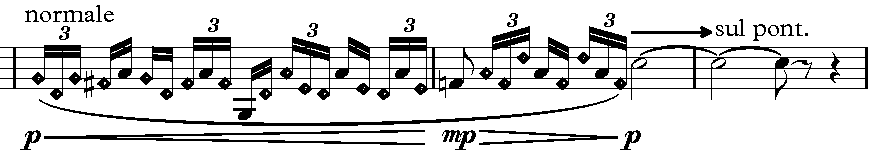
\includegraphics[width=\linewidth]{./resources/violinHalfHarmonicsExcerpt5.pdf}
    \caption{mm.\@ 5--7 of \violinPiece}\label{fig:Excerpt from what are you doing with the humans, mm. 5}
  \end{figure}

In \autoref{fig:violin31}, I use the D string to provide additional available harmonics; the fifth D string harmonic, octave D string harmonic, and a fourth artificial harmonic using a stopped A are all readily available underneath the violinist's fingers.
\begin{figure}
  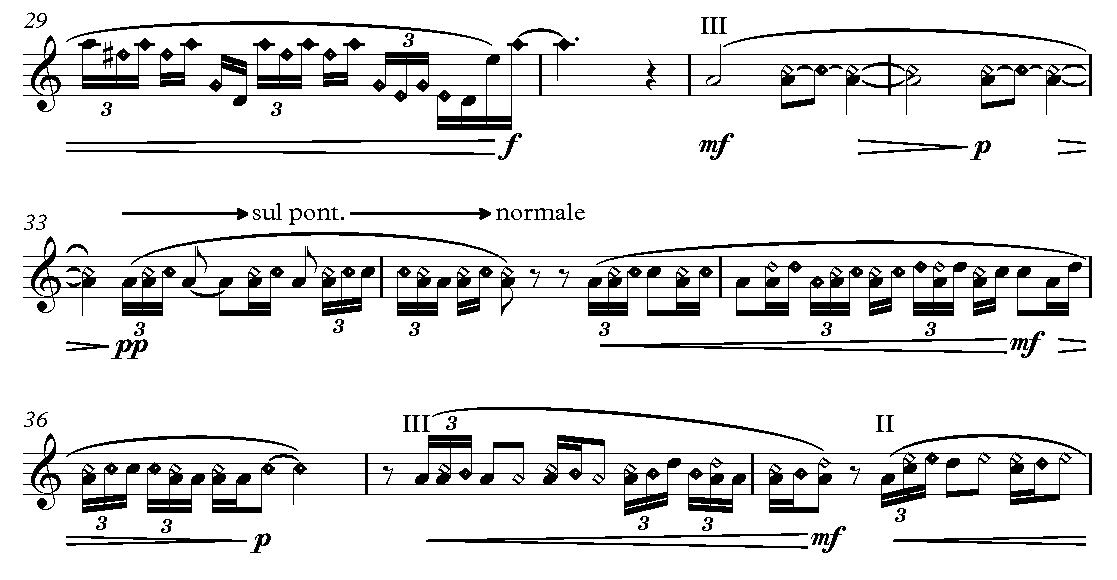
\includegraphics[width=\linewidth]{./resources/violinHalfHarmonicsExcerpt31.pdf}
  \caption{mm.\@ 29--36 of \violinPiece}\label{fig:violin31}
\end{figure}

Thus, the difficulty is not in the fingering on the fingerboard, but the quick changes between harmonic, half-harmonic, \emph{normale}, and artificial harmonic.
Through this facet of eliminating needless complexity, the work serves as an etude targeting specifically the production of half-harmonics.

\violinPiece\space takes inspiration from Sciarrino's \hyperref[fig:sciarrinoExcerpt]{fifth Caprice}, and serves as a stepping stone to the more difficult work.\autocite[]{sciarrinoCapricciViolino1976} 
In practice, the pitch content of my work was obscured by the noisy texture of half-harmonics, rendering large portions of it as noise. 
With the knowledge that properly performed, the harmonic content would be obscured, I leant into this, writing in a more tonal style than I do usually.

I opted to omit specific string instructions for the majority of the work, as this work is at a difficulty level where players should be able to make intelligent decisions over which strings to use.
Where a natural harmonic is desired specifically, and not an artificial harmonic, the fundamental has been notated with a small notehead in parentheses. 

As the technique is available on both nodal points, and non-nodal points (i.e.\ the technique is not limited to the fingering positions of harmonics on each string), I wanted to clearly delineate this with a section comprised of half-harmonics that do not excite any harmonics, shown in \autoref{fig:halfHarmonicNotOpen}. 
The timbre of these non-nodal half-harmonics is darker than the others, and they are more difficult to speak.\autocite[]{smithFeedbackCelloSightreading2019}
\begin{figure}
  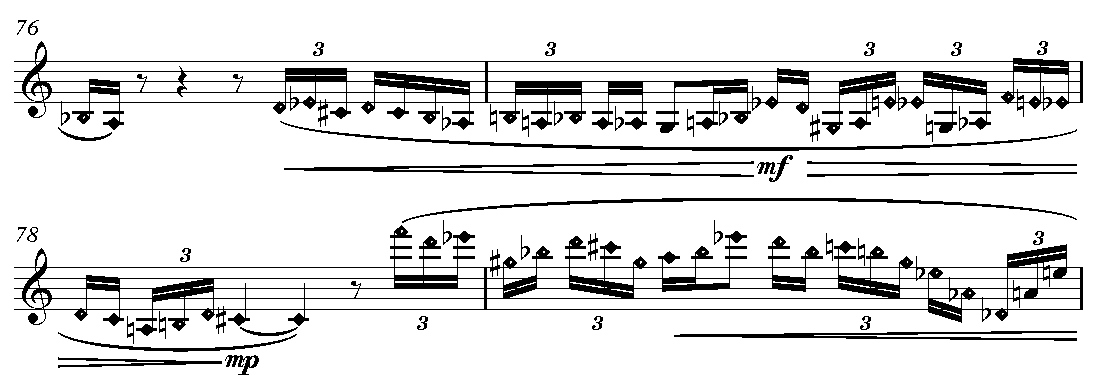
\includegraphics[width=\linewidth]{./resources/halfHarmonicNotOpen.pdf}
  \caption{mm.\@ 73--79 of \violinPiece}\label{fig:halfHarmonicNotOpen}
\end{figure}


I explore the inverse of this, playing on nodes to bring out the harmonic content as seen in \autoref{fig:halfHarmonicOpenStringsExcerpt}.
Here, \emph{normale} open string notes (for the most part) signal the end of the use of the string; in this way, the player will learn how to make the half-harmonics speak properly while moving the bow to different strings.

\begin{figure}
  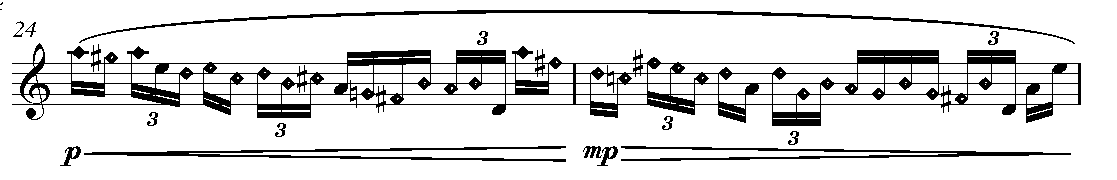
\includegraphics[width=\linewidth]{./resources/halfHarmonicOpenStringsExcerpt.pdf}
  \caption{mm.\@ 24 of \violinPiece}\label{fig:halfHarmonicOpenStringsExcerpt}
\end{figure}

Another facet of half-harmonics that I wanted to explore was the timbral aspect of them, bar 27 shown in Figure~\ref{fig:violinHalfHarmonicsExcerpt27}.
Similar to a multiphonic in their rich harmonic content, half-harmonics do not have the purity of tone that regular harmonics have, and are more often a type of multiphonic, as evidenced by Fallowfield's example.\autocite[]{fallowfieldCelloMapHalf2013}
% TODO: Fallowfield half-harmonics example - https://trello.com/c/A4Awcmxz/30-fallowfield-half-harmonics-example
I explore the interplay of half-harmonics, regular harmonics, and \emph{normale}, double stopped minims and semibreves slowly changing from one mode of pressure to another.
In this way, violinists that play \violinPiece\space will become familiar with different modes of pressure played concurrently.

\begin{figure}
    
\includegraphics[width=\linewidth]{./resources/violinHalfHarmonicsExcerpt27.pdf}
    \caption{Excerpt from \violinPiece}\label{fig:violinHalfHarmonicsExcerpt27}
  \end{figure}

Notationally, the rapid changes between half-harmonics and other techniques were an ideal testing ground for different notation types.
Notably, the issue of half-filled diamond noteheads not having any distinction between crotchets and minims is not an issue due to the bulk of the work dealing in smaller divisions of the beat.\footnote{Which is to say, that the connection of stems make the timing obvious for quaver and smaller noteheads, regardless of the notehead.}
The considerations of how to best notate half-harmonics are discussed further in \autoref{sec:notation-half-harmonics}.

Ultimately, I opted to implement the half-filled diamond noteheads, finding them to most accurately present the information in a way that was unobtrusive, and built upon pre-existing notation.
It should be noted that this is contrary to the opinion set out in Dimpker's seminal thesis on notation, \emph{Extended notation. The depiction of the
unconventional}, but conforms to Gould's opinion on the matter.\autocites[120--121]{dimpkerExtendedNotationDepiction2012}[61]{gouldBars2011}
% TODO: fix gould citation - https://trello.com/c/gYLN8lqN/28-fix-gould-citation


\section{\violaPiece}\label{sec:violaPiece}
% TODO: Write Doppelganger
\hyperref[app:violaPiece Score]{\violaPiece} is a piece for solo viola, written to explore the lower register of the viola using \hyperref[sec:subharmonicsDiscussion]{subharmonics} juxtaposed with upper harmonics. 
The pitch distance between subharmonics and harmonics sidestep the viola's usual role occupying the middle register.



\subsection{Findings of \violaPiece}

Workshopping an early draft of \violaPiece\space with \violaParticipant, I found that subharmonics came fleetingly, and were prone to `jump back' to the fundamental.\autocite[]{appleseedFeedbackExploratorySession2019}
This resulted in a rewrite, redirecting the focus of the technique as a more textural element. 
As such, I amended the score to treat subharmonics largely as a `special effect', and not ascribe importance to their pitched content.

A second workshop with \violaParticipant\space was more productive, and we found that the subharmonic technique spoke much more readily with a slower bow speed, combined with a consistent amount of pressure.\autocite[]{appleseedFeedbackSightreadingSession2019}
We found that the A string of the viola did not respond nearly as readily to the technique, to the point of being unusable.
The D and G strings both spoke acceptably, but due to the pressure required, often resulted in unwanted double-stopping.
The C string spoke very freely, with the technique coming readily.
Contrary to Fallowfield stating `It is very difficult to sustain the tone, which often has a high noise component', we found that with practice, the subharmonic was able to stabilise to the point of it being usable for longer sustained notes.\autocites[http://www.cellomap.com/index/the-string/plucking-striking-and-bowing-the-string/how.html]{fallowfieldCelloMapHandbook2009}[]{fallowfieldCelloMapExample2013}[]{appleseedFeedbackSightreadingSession2019}

To `ease the player into' the technique, \violaPiece\space begins with an open C string, which drones for a few seconds before crescendoing while moving the bow towards the fingerboard and slowing the bowing speed down, shown in \autoref{fig:doppelgangerStart}.
\begin{figure}
  \centering
  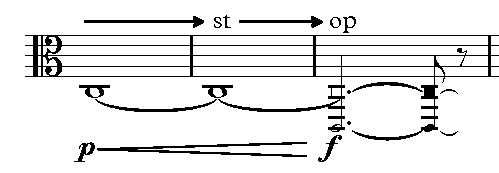
\includegraphics{./resources/doppelgangerStart.pdf}
  \caption{mm.\ 1--3 of \violaPiece.}\label{fig:doppelgangerStart}
\end{figure}
The pressure used to play \emph{sul ponticello} is the same as the pressure needed to play subharmonics, priming the player to only need to concentrate on the bow speed and location on the string.\autocite[]{appleseedFeedbackSightreadingSession2019}
This technique of applying the thought process of playing \emph{sul tasto}, but actually playing near the fingerboard appears to be an ideal way to guide players unfamiliar with the technique into achieving it without lengthy in-person demonstrations.\autocites[]{appleseedFeedbackSightreadingSession2019}{bloggsFeedbackContrabassSession2019}

\section{\celloPiece}\label{sec:celloPiece}

\hyperref[app:celloPiece Score]{\celloPiece} is an exploration in multiphonics, but is not strictly an etude.
I discovered several facets of the technique that were not previously discussed in the literature found in Fallowfield's work.\autocite[]{fallowfieldCelloMap}
I wanted to explore multiphonics as I explored \hyperref[sec:half-harmonics]{half-harmonics} in the piece \autoref{sec:violinPiece}, shifting between \emph{normale} and the technique.
Unfortunately, while workshopping with \celloParticipant, I found the non-binary nature of multiphonics precluded this from being a possibility; the multiphonics speak on a sliding scale, and controlled attempts to shift between the two sound as though they are just failing to speak.\autocite[]{smithFeedbackCelloSightreading2019}


For each pair of nodes that produce multiphonics, the lower of the two is easier to pitch due to the logarithmic correlation between string length and pitch;
that is to say, because the gaps between semitones are correlationally larger as the pitch lowers, the pitching can be more precise.

Double-stopped multiphonics are feasible, but because the angle of attack can impact the partials the multiphonic produces, the shift between single strings and double stopping can stop the multiphonic from speaking clearly.\autocite[]{smithFeedbackCelloSightreading2019}
Aurally, double stopped multiphonics seem to be more effective with the \emph{normale} note on a lower string than the multiphonic.



\section{\bassPiece}\label{sec:bassPiece}
% TODO: Write The Veldt
Inspired by the eponymous short story by Ray Bradbury, \hyperref[app:bassPiece Score]{\bassPiece} is a composition for solo contrabass that explores both \hyperref[sec:multiphonicsDiscussion]{multiphonics} and \hyperref[sec:subharmonicsDiscussion]{subharmonics} in the context of a soundworld; the musical language is derived from the harmonic series, exploiting the resonance of the bass to maintain a drone.\autocite[]{bradburyVeldt1951}
Similarly like the plot of Bradbury's work, this world is filled with danger but also beauty. 
This is reflected in my work in the use of subharmonics and multiphonics; difficult and fragile techniques that can break at a moments notice, inspired by Thurley's treatment of multiphonics in \emph{yet another example of the porousness of certain borders}.\autocite[]{thurleyAnotherExamplePorousness2014}
My intent with Veldt was to create a harmonic language and space that the performer was able to `roam around' in, and features several sections of improvisation or stochastic aleatory based around the harmonic series, representing the possibilities of the veldt.

\subsection{Findings of \bassPiece}
Writing for contrabass and experimenting on my own bass, I found subharmonics came most easily on the G string. 
This was confirmed in a workshop with \bassParticipant, although he was able to produce subharmonics on all other strings, too.
Subharmonics on the lower strings did not speak as well, and it was difficult to discern the lower frequency's shifts.
Because of this, \bassPiece\space uses the technique as a textural tool, rather than a melodic device.
% They translate well into animalistic 

Working with \bassParticipant, he identified the need for subharmonics to be played closer to the fingerboard than normal.
He theorised that the tension being weaker as the contact point moved away from the bridge, closer to the middle, made it easier to produce subharmonics via the raucous motion.\autocite[]{bloggsFeedbackContrabassSession2019}
A second stave displaying the music notated at actual pitch was necessary, as shown in \autoref{fig:multiphonicsBassExample}.
\begin{figure}
  \centering
  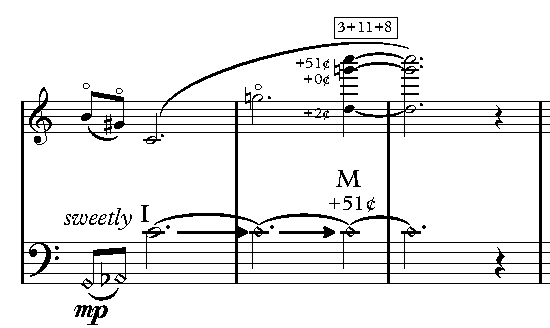
\includegraphics{./resources/multiphonicsBassExample.pdf}
  \caption{excerpt from \bassPiece\space showing the \emph{suono reale} stave.}\label{fig:multiphonicsBassExample}
\end{figure}
\begin{figure}
  \centering
  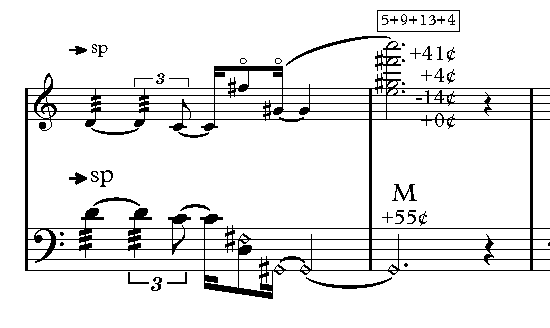
\includegraphics{./resources/multiphonicsFingeringExample.pdf}
  \caption{Excerpt from \bassPiece.}\label{fig:multiphonicsFingeringExample}
\end{figure}
In contradiction of Gould's recommendations, I opted to notate the \emph{suono reale} in treble clef, rather than treble transposed down an octave.\autocite[423]{gouldBars2011}
This is because the multiphonics activate partials well above those usually expected, resulting in the advice not being relevant.

To maintain ease of playing, I use similar fingerings across the strings to aid in the pitching of multiphonics, as seen in \autoref{fig:multiphonicsFingeringExample}.





% I was inspired greatly by Oliver Thurley's \emph{yet another example of the porousness of certain borders}, whose treat\autocite[]{thurleyAnotherExamplePorousness2014}

% % chapter4.tex (Chapter 4 of the thesis)

\chapter{Findings and Research Implications}\label{ch:chapter4}
%%??? My findings are presented as a manual  ...   findings from each piece singularly.
In this chapter, my findings are presented as an instructive manual for composers and performers interested in using the techniques.
Because my folio of works has some degree of overlap in usage of techniques, this chapter will deal with each technique, rather than be a review of findings from each piece singularly.
% Where relevant, I will include my findings from working with performers.
%%??? The folio of works discusses the usage of techniques;  rather than recapitulate these points, this chapter primarily reviews 


%%??? How about: The Dick model of categorisation (NOTE SPELLING) will not be discussed due to its relative lack of use, limited applicability and notational challenges.
Due to the limited number of permutations of these techniques, the Dick model of categorisation will not be discussed due to its limited applicability and the notational challenges of these techniques.\autocite{dickOtherFlute1989} 
It will also take into account how common the technique is, as well as notational challenges.

\subsection{Notation}
If a composer wishes to use a technique once off, or in sparing amounts, plain English text explaining the technique and what is desired of the player is adequate..\autocite[494]{gouldBars2011}
For all other cases where a technique is required more than once, composers should include the technique in the frontmatter of the work.\autocite[494]{gouldBars2011}
If a technique uses a new symbol or notehead, this should be reflected in the frontmatter.
Where possible, composers should retain the same clef for both fingered and sounding pitches.\autocite[422]{gouldBars2011}

Composers would do well to include a description of the desired sound, and method of production, as shown in the frontmatter for each of my works. \begin{itemize}
  \item Subharmonics: \begin{itemize} 
    \item \hyperref[app:violaPiece Score]{\violaPiece} 
    \item \hyperref[app:bassPiece Score]{\bassPiece} \end{itemize}
  \item Multiphonics: \begin{itemize} 
    \item \hyperref[app:bassPiece Score]{\bassPiece} 
    \item \hyperref[app:celloPiece Score]{\celloPiece}\end{itemize}
  \item Half-harmonics: \begin{itemize} 
    \item \hyperref[app:violinPiece Score]{\violinPiece}\end{itemize}
\end{itemize}
% example frontmatter is provided for each of the techniques, \hyperref[sec:subharmonicFrontmatter]{subharmonics}, \hyperref[sec:multiphonicFrontmatter]{multiphonics}, and \hyperref[sec:halfHarmonicFrontmatter]{half-harmonics}. 


\section{Subharmonics}\label{sec:subharmonics}
Subharmonics are a difficult technique that lend themselves to solo works, or works where they can be brought to the forefront.
They produce a sound lower than the fundamental through precise control of torsional oscillation, which usually produces the sound of an amateur string player's heavy handed, slow bowing. 
The timbre of overpressure can vary, but is identifiably pitched, and typically is somewhat nasal.
Subharmonics are notably different to overpressure, but bleed over into non-pitched overpressure is common.
This, plus the difficulty in their execution, makes them unsuitable for melodic content.

Several different intervals are available as subharmonics and a myriad of factors feed into which are easily replicable. As a rule, octaves come most easily, with minor seconds, major sevenths, and perfect fifths coming after that.\autocite[]{kimuraHowProduceSubharmonics1999}
Composers should be aware that producing the specific pitch is not \emph{necessarily} guaranteed.
Subharmonics are unable to be performed \emph{laissez vibrer}, as the pitch returns to the fundamental as soon as the bow is no longer in contact with the string.\autocite[]{appleseedFeedbackExploratorySession2019}
Due to the pressure needed, subharmonics are most comfortable at least \emph{mezzo-forte} or louder, although quieter subharmonics are possible. 
Sympathetic resonances from the other strings are common at higher volumes.
Playing on the two inner strings is slightly harder due to the angle of attack being restricted to not inadvertently play double-stopped notes.\autocite[99]{welbanksFoundationsModernCello}



Composers looking to use this technique should be aware that instrumentalists will need copious amounts of practice and guidance in order to fully and reliably realise this technique.

\subsection{Notation of Subharmonics}\label{sec:notation-subharmonics}
% Subharmonics should be notated with a square notehead, and a small notehead (optionally in parenthesis) at the desired pitch.
Subharmonics require both a fingered pitch, and an intended resultant pitch to be conveyed to the player, as well as some form of indication that it is a subharmonic.
This can be done through a variety of ways, including technique text (i.e.\ `S.H.' as Long suggests), or using a different notehead.\autocite[]{longSubharmonics2019}

Gould suggests several practical methods of communicating resultant pitch, as a ``small [black] notehead [without a stem] in brackets directly above or after the fingered pitches'', an ossia stave with the resultant pitches above, or notated in a footnote using a cue stave.\autocite[421]{gouldBars2011}
She states ``wherever possible, retain the same clef for both fingered and sounding pitches'', though this is sometimes impractical.\autocite[422]{gouldBars2011}
% This is sometimes practical, but gives rise to the issue of indicating pitch. 
The use of a second stave is seen in \autoref{fig:Excerpt from Risset's Variants}.\autocite[It should be noted that Risset's notation omits a fingered pitch, which is not recommended.]{rissetVariants1995}
Extrapolating from the use of the circular harmonic signifying at-pitch harmonics, we can apply the same method to subharmonics, as seen in \autoref{fig:subharmonicsNotationExampleTwoStave}.
\begin{figure}
  \centering
  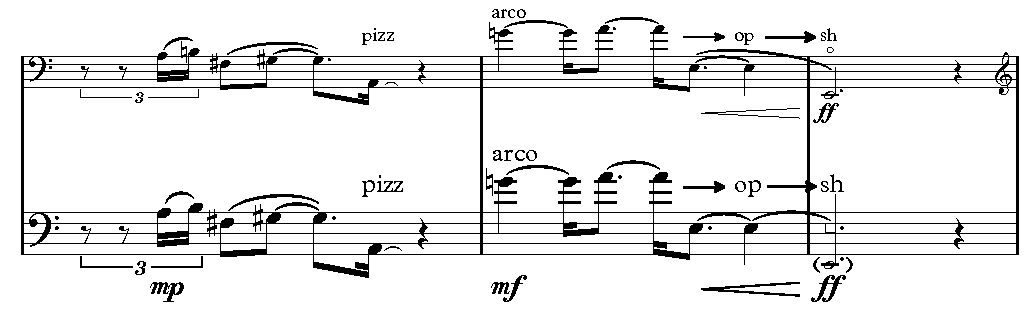
\includegraphics[width=\linewidth]{./resources/subharmonicsNotationExample.pdf}
  \caption{Excerpt from \bassPiece\space showing subharmonics notation.}\label{fig:subharmonicsNotationExampleTwoStave}
\end{figure}


\subsection{Observations on techniques} %%??? itemize?
\begin{itemize}
 \item Rope core strings produce more harmonics, but are more difficult to produce subharmonics with.
 \item Strings with a single or nylon core make the technique easier, due to their low tension.\autocite[99]{welbanksFoundationsModernCello}
 \item Players may find that subharmonics are easier on older strings.\autocite[]{kimuraHowProduceSubharmonics1999}
 \item They may also find that adding twists to the string may also help, or hinder the production of subharmonics, as shown in \autoref{tab:twistTable}.\autocite[]{kimuraHowProduceSubharmonics1999}
\end{itemize}



Botting notes that experimentations with octavic subharmonics yielded a pitch slightly flatter than an octave. He states: \begin{quotation}
  I developed a left hand finger technique whereby I rotate my hand slightly clockwise, pivoting on the finger stopping the string, which has the effect of sharpening the subharmonic enough to be more in tune with the fundamental.\autocite[111]{bottingDevelopingPersonalVocabulary2019}
\end{quotation}

To `find' the subharmonic, an excellent method to practice is to play \emph{sul ponticello} at a \emph{forte} dynamic on an open string, and then move towards the fingerboard, keeping the pressure but slowing the bowing speed down.
Subharmonics are easier to find at nodal points\footnote{Points at which the string is divided into fractional ratios, such as 1/3.}, particularly the 6th node (closest to the bridge).\autocite[]{appleseedFeedbackSightreadingSession2019}
Bow pressure should be totally consistent throughout the bowing stroke; rather than the tapered start and finish of \emph{normale}, players should imagine a more binary stop and start, beginning and ending on the string.
The bow hair should remain flat throughout the stroke, in order to to exert the maximum amount of pressure.\autocite[]{kimuraHowProduceSubharmonics1999}
Different bow positions on the string can make different subharmonics speak more easily.\autocite[]{kimuraHowProduceSubharmonics1999}

\subsubsection{Instrument specific considerations for subharmonics}
Subharmonics may be easier to produce on the contrabass with a lighter bow, preferably a cello bow, or alternatively a French style bow.\autocite[]{longSubharmonics2019}
Conversely, violin and violas may benefit from the use of a heavier bow.\autocite[]{appleseedFeedbackSightreadingSession2019}
The A string of the viola appears to be particularly resistant to producing subharmonics, although this may vary from instrument to instrument.\autocite[]{appleseedFeedbackSightreadingSession2019}
The tension of the string appears to impact the feasibility enormously; 13 inch violas may have more success producing subharmonics on the A string than 18 inch violas.\autocite[]{appleseedFeedbackSightreadingSession2019}


%%??? I suggest moving the discussion of notation to the start of the chapter, followed by a section "Observations on techniques" which is constituted by the preceeding subsections
%%??? as itemised blocks 


% TODO: Example of Subharmonics --- https://trello.com/c/bc3sNJTL/32-example-of-subharmonics


% \subsubsection{Subharmonic Frontmatter}\label{sec:subharmonicFrontmatter}

\subsection{Works featuring subharmonics }\label{sec:subharmonicsLiterature}

\begin{itemize}
    \item Mari Kimura --- ALT in three movements for solo violin (1992)
    \item --- Gemini for solo violin (1993)
    \item --- 6 Caprices for subharmonics for solo violin (1997) 
    \item --- JanMaricana (for subharmonics) for solo violin (2016)
    \item Joshua Burel --- Sonata No. 2 for violin and piano `Subharmonics' (2011)
    \item Jean-Claude Risset --- Variants (1995)
    \item Robert Rowe --- Submarine (1996)
\end{itemize}


%%??? Again notation ought to precede  the implementation

\section{Multiphonics}\label{sec:multiphonics}

Multiphonics are fragile, and require much practice to execute reliably.
Despite this, they can be used to achieve harmonies that are not otherwise achieveable through double-stopping, and lend themselves well to drawn out or slow passages of music. 
Multiphonics' exact pitching makes them ideal for music that uses ratios, microtones, or tone rows. 
Multiphonics are easier to achieve on larger instruments, due to the need for precise ratio-based fingering to achieve the resonance of multiple partials.\autocite[http://www.cellomap.com/index/the-string/multiphonics-and-other-multiple-sounds/frequency-analysis.html]{fallowfieldCelloMap}

The open string (or first partial) can be activated as part of a multiphonic.\autocite[161]{welbanksFoundationsModernCello}
The second partial (octave harmonic) is \emph{never} produced in a multiphonic

\subsection{Notation of Multiphonics}\label{sec:notation-multiphonics}
Much has been written about multiphonics, and they are a well established technique in woodwind writing.
The notation between them differs, though; precise fingering charts above resultant pitches do not translate precisely into string writing.\footnote{The relation between string and woodwind multiphonics is discussed more in-depth \hyperref[sec:multiphonicsWoodwind]{in chapter 2.}}
Fallowfield states: \begin{quotation}
    To notate ‘pure’ multiphonics accurately in a score, however, it is necessary to indicate both the left-hand finger position and the pitch content. 
    The left-hand finger touches the string above the node of the highest harmonic that contributes to the multiphonic, so the finger position is always that of the highest harmonic in the group. 
    I suggest notating finger position with the rhombus that is usually used for harmonic finger pressure. 
    The pitch of the contributing harmonics could be notated in brackets or on a separate stave.
    It is necessary to indicate which string the multiphonic should be played on and helpful to use the indication ‘M’ for multiphonic.\autocite[http://www.cellomap.com/index/the-string/multiphonics-and-other-multiple-sounds.html]{fallowfieldCelloMap}
\end{quotation}
Below, I have notated the permutations of what Fallowfield has described, and will let the reader draw their own conclusion as to which is most appropriate.
Her example omits the necessary string, but Gould suggests several different options; the inclusion of the corresponding string number (i.e.\ `I', `IV'), the usage of Italian (i.e.\ `sul E', `sul G'), or by notating the fundamental on the stave, using ``a small bracketed black notehead (regardless of duration) for the open string and for the first note only of a tied harmonic''.\autocite[418]{gouldBars2011}
In \autoref{fig:multiphonicNotationCent}, we see the specific cents tuning for the fingered note, contrasted with \autoref{fig:multiphonicNotationQuarter}, which uses quarter tones to convey the relevant pitching data, both with a \emph{suono reale} stave indicating the sounding pitch above.

\begin{figure}
  \centering
  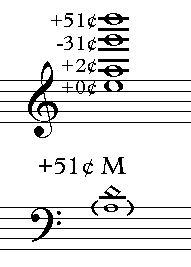
\includegraphics{./resources/multiphonicNotationCent.pdf}
  \caption{Multiphonic notation with cents}\label{fig:multiphonicNotationCent}
\end{figure}

\begin{figure}
  \centering
  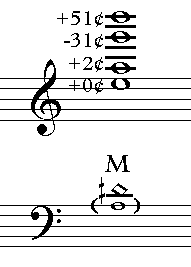
\includegraphics{./resources/multiphonicNotationQuarter.pdf}
  \caption{Multiphonic notation with quarter tones}\label{fig:multiphonicNotationQuarter}
\end{figure}
While \autoref{fig:multiphonicNotationCent} is more precise, the horizontal space usage is greater than that of \autoref{fig:multiphonicNotationQuarter}; if using text to specify which string to use, it may quickly become cumbersome to read.


Gould's advice for resultant pitch for harmonics, which has been applied to subharmonics can also be applied to multiphonics as evidenced in \autoref{fig:multiphonicNotationOneLine}
The ossia staff, or \emph{suono reale} if necessary for the entirety of the work\footnote{\emph{suono reale} should be full sized, while ossia staves are 3/4 sized.}, can have the multiphonics notated as a rhythm, as seen in \autoref{fig:multiphonicNotationOssia}.

\begin{figure}
  \centering
  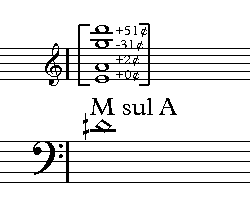
\includegraphics{./resources/multiphonicNotationOssia.pdf}
  \caption{Multiphonic notation using an ossia line}\label{fig:multiphonicNotationOssia}
\end{figure}

\begin{figure}
  \centering
  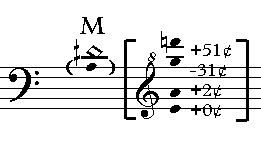
\includegraphics{./resources/multiphonicNotationOneLine.pdf}
  \caption{Multiphonic notation on one line}\label{fig:multiphonicNotationOneLine}
\end{figure}

Further simplifications can be made if there is no clef change, making it possible to omit the `M' technique text denoting it as a multiphonic.

\begin{figure}
  \centering
  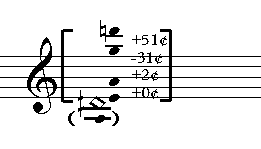
\includegraphics{./resources/multiphonicNotationOneLineClef.pdf}
  \caption{Multiphonic notation in one clef}\label{fig:multiphonicNotationOneLineClef}
\end{figure}

There are several ways of denoting the same (or similar) information; because multiphonics notation is cumbersome, there is often a deficit of either vertical or horizontal space.
However, with the flexibility of each element, there should be a method of notating multiphonics idiomatically that can be implemented in every score that makes use of them.


\subsection{Observations on techniques}
%%??? the following bits could be itemized
\begin{itemize}
  \item Multiphonics should be played closer to the bridge than one would normally play them.\autocite[]{fallowfieldCelloMap}
  \item Overly high and low bow pressure can limit the lower partial content of resultant multiphonics.
  \item Faster bow speed favours higher partials over lower partials, and similarly, slower bow speed favours lower partials over higher.
  \item Moving the contact point closer to the bridge yields more noise content and favours lower partials, until the contact point is very close to the bridge, where it produces a clearer sound and favours higher partials over lower partials.\autocite[http://www.cellomap.com/index/the-string/multiphonics-and-other-multiple-sounds.html]{fallowfieldCelloMap}
  \item Multiphonics containing higher partials require a lighter and faster bow stroke, closer to the bridge than multiphonics that have lower ranges of partials.\autocite[165]{welbanksFoundationsModernCello}
\end{itemize}


To first find a multiphonic, Welbanks and Fallowfield both recommend playing the harmonics individually.\autocite[167]{welbanksFoundationsModernCello}
Then play the harmonic with the highest resultant pitch. 
Use a slower bow stroke with higher pressure and closer to the bridge, and slightly lighter finger pressure.


\subsubsection{Instrument specific considerations for multiphonics}
Multiphonics are easier on large instruments, as more precise pitching is possible with the longer strings.
Composers should be aware that of the pair, the multiphonic node closer to the bridge can be harder to produce because of this fact.
`Artificial' multiphonics are possible, although much more difficult.\autocite[772]{guettlerBowedstringMultiphonicsAnalyzed2012}


% \subsubsection{Multiphonic Frontmatter}\label{sec:multiphonicFrontmatter}
% \begin{quotation}
  
%   Multiphonics are achieved through clusters of close harmonic nodes, and by playing a harmonic close to the highest partial.
%   Note that not all of these pitches will actually sound in practice.
  
%   Multiphonics are notated as a harmonic position using a diamond notehead, with an `M' above the note to be fingered.
%   Where the string used is ambiguous, it is notated below the sounding pitch as a small, bracketed notehead.
%   Precise tuning is given in cents, and unless otherwise notated, is intended for the first note that the multiphonic is attached to.\footnote{100 cents is equal to a semitone. Therefore, +51c is roughly equal to half a semitone sharp. Cents have been used due to their precision compared to more granular accidentals such as the quartertone sharp.}
%   The theoretical sounding pitches are given in a bracketed staff above the main stave.
%   % Above the sounding pitches, the sounding partials are given (i.e. M IV [4th + 13th + 9th + 15th + 5th]).

%   The bow should exert slightly more pressure than usual and should be drawn with a consistent speed which should be slower than for harmonics.
%   The location of the bow can encourage or discourage upper or lower partials, and experimentation should be done during the practice of this work to achieve the pitches desired.
% \end{quotation}


\subsection{Works featuring multiphonics}\label{sec:multiphonicsLiterature}
% TODO: Find multiphonic works --- https://trello.com/c/o75LaLo8/13-find-multiphonic-works

\begin{itemize}
    \item Mari Kimura --- 6 Caprices for subharmonics for solo violin (1997) 
    \item Andrew Greenwald --- On Structure (2a) --- for clarinet, violin, and cello (2010)
    \item Stefano Scodanibbio --- composed e/statico (1980)
    \item Håkon Thelin --- oibbinadocS (2004)
    \item --- Glasperlenspiel (2010)
    \item Michael Liebman --- Sonata for double bass, movement 2: Legato sonore (2001)
    \item Kaija Saariaho --- Lichtbogen (1986)
    \item Kimmo Hakola --- Thrust, Rubato (1989, rev. 1991) 
    \item Eivind Buene --- `Blacklight' (2019)
    \item Fernando Grillo --- `Fluvine' (1974)
% Brian Ferneyhough Trittico Per G.S
% Iannis Xenakis' \emph{Theraps} for solo contrabass is \lipsum[1].\autocite[]{}
% Barry Guy Statements II
\end{itemize}

\section{Half-harmonics}\label{sec:half-harmonics}
Half-harmonics are produced via left-hand finger pressure that is halfway between that of a harmonic and a \emph{normale} sound produced when the string is pressed to the fingerboard.
The pitch content is sharpened slightly, and the overtone content is relatively weak.\autocite[113]{welbanksFoundationsModernCello}
Half-harmonic stops are not limited to the nodes and hence the natural harmonics, but may be executed on all fingerboard positions, as well as executed as `artificial' harmonics.\autocite[127]{dimpkerExtendedNotationDepiction2012} 
Half-harmonics are what many would interpret as notes that `fail to speak'.


\subsection{Notation of Half-harmonics}\label{sec:notation-half-harmonics}
Half-harmonics can be notated in one of several ways (see \autoref{fig:halfHarmonicNotationExamples} for examples of both the crotchet and semibreve notation of each), but regardless of the chosen symbol, the notation should be described in the performance notes.

\begin{figure}
    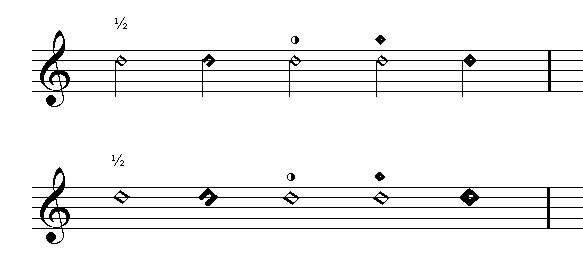
\includegraphics[width=\linewidth]{./resources/halfHarmonicNotationExamples.pdf}
    \caption{Half-harmonic notation examples}\label{fig:halfHarmonicNotationExamples}
\end{figure}

  
The simplest method, using text rather than a graphic may produce good results, as seen in \autoref{fig:textSymbolNotation}.
No scores appear to use this method, despite it being the only example able to convey more precise ratios of finger pressure as Fallowfield states is possible.\autocite[http://www.cellomap.com/index/the-string/multiphonics-and-other-multiple-sounds/other-multiple-sounds.html]{fallowfieldCelloMap}

\begin{figure}
  \includegraphics[page=1,width=\textwidth]{resources/halfHarmonicsSingleExamples.pdf}
  \caption{Half-harmonic displayed with text}\label{fig:textSymbolNotation}
\end{figure}

The second and last of the examples in \autoref{fig:halfHarmonicNotationExamples} do not have discrete noteheads for crotchets and minims like regular diamond noteheads.
As such, if there is rhythmic ambiguity, rhythms should be clarified above the stave as normal.
The second example, as seen in Sciarrino's \emph{Six Capricci for Violin} (\autoref{fig:sciarrinoExcerpt}) shows the ambiguity of this.
The `slant' of the regular harmonic notehead is opposite to the unfinished diamond, going from up to down, helping distinguish it.

The third example unfortunately is not without issues, either; (\emph{normale}) harmonics denoted with a circle are exclusively for the resultant pitch.\autocite[419]{gouldBars2011} 
While half-harmonics do produce the notated pitch, rapid transitions between half-harmonics and \emph{normale} harmonics using half-filled circles may cause confusion due to the translation between a symbol that denotes pressure needed and a resultant harmonic respectively, as illustrated in \autoref{fig:circleExample}, which is the notation used for half-depressed valves on brass instruments.\autocite[85]{cherryExtendedTechniquesTrumpet2009}
This is compounded by the circle notation's inability to handle harmonics that fall well outside the range of the staff (i.e.\ major 3rd and minor 3rd harmonics), resulting in a need for at least two types of notation; circular half-harmonics, and diamond noteheads for problematic \emph{normale} harmonics.

\begin{figure}
    \includegraphics[page=3,width=\textwidth]{resources/halfHarmonicsSingleExamples.pdf}
    \caption{Half-harmonic circular notation}\label{fig:circleExample}
  \end{figure}

The fourth example of notation displayed in \autoref{fig:diamondSymbolNotation} is a non-standard symbol, and also suffers the same issues that plague the previous example.

\begin{figure}
  \includegraphics[page=4,width=\textwidth]{resources/halfHarmonicsSingleExamples.pdf}
  \caption{Half-harmonic diamond symbol notation}\label{fig:diamondSymbolNotation}
\end{figure}


Compare this with \autoref{fig:halfFilledNotation} and \autoref{fig:halfEmptyNotation}, which is an example of Sciarrino's half-empty notation as seen in \autoref{fig:sciarrinoExcerpt}.

\begin{figure}
  % \includegraphics[width=\linewidth]{./resources/circleExample.pdf}
  \includegraphics[page=5,width=\textwidth]{resources/halfHarmonicsSingleExamples.pdf}
  \caption{Half-harmonic half-filled notehead}\label{fig:halfFilledNotation}
\end{figure}


\begin{figure}
  % \includegraphics[width=\linewidth]{./resources/circleExample.pdf}
  \includegraphics[page=2,width=\textwidth]{resources/halfHarmonicsSingleExamples.pdf}
  \caption{Half-harmonic half-empty notehead}\label{fig:halfEmptyNotation}
\end{figure}



Observe that neither the half-filled notehead as depicted in Gould and \autoref{fig:halfFilledNotation}, nor the Sciarrino style half-empty notehead as seen \autoref{fig:halfEmptyNotation} are available in modern versions of Sibelius or Dorico as of the time of writing.\autocite[424]{gouldBars2011}
The flagship Standard Music Layout Font (SMuFL), Bravura, includes the half-harmonic circle as depicted in \autoref{fig:circleExample}, but is only available on Dorico and the Sibelius port of Bravura, Norfolk.\autocite[]{w3ccommitteeStandardMusicFont2019}


\subsection{Observations on techniques}
Half-harmonics are pitched slightly sharp, and so should be fingered accordingly flat to compensate for this.\autocite[113]{welbanksFoundationsModernCello}

% \subsubsection{Half-harmonic Frontmatter}\label{sec:halfHarmonicFrontmatter}
% Half-harmonics are produced by applying left hand finger pressure halfway between that required to create a harmonic, and a \emph{normale} sound. 
% The sound that is produced should be a mixture of the stopped string pitch, the harmonic pitch, and a resistant, slightly noisy quality.
% They are notated in the score as a half-filled diamond notehead.
\subsection{Works featuring half-harmonics}\label{sec:half-harmonicsLiterature}

\begin{itemize}
    \item Robert Rowe --- Flood Gate (1989)
    \item Salvatore Sciarriono --- 6 Capricci for violin (no. 5) (1976) 
    \item Helmut Lachenmann, Gran Torso
    \item Trevor Bača --- Al-Kitab Al-Khamr (2015)
    \item Claudio Pompili --- Scherzo Alla Francescana (1990, revised 1994)
    \item Mary Bellamy --- Transference (?)
    \item Sam Park --- The Colour of Light (2010)
    \item Jack Symmonds --- Hell Is Murky (2018)
    \item Mark Applebaum --- The Plate of Transition Nourishes the Chameleon Appetite (1992, revised 1994)
    \item Henrik Deneren --- seals II (2014--15)
    \item Ramteen Sazegari --- Slate Representative (2015)
\end{itemize}
% Conclusion
% These techniques are underrepresented because of a variety of reasons, one of them being that there is a lack of resources dedicated to writing for them.
% It is hoped that this exegesis will contribute to their more widespread adoption. 
% It becomes apparent that the literature surrounding these techniques still lacks comprehensive guidelines over the techniques' use, and the works that have been produced have been through trial and error.
\section{Impact and Further Research}
\emph{The author of a compendium on modern instrumental technique faces the disconcerting prospect that as soon as his tabulation is published, it is likely to be considered incomplete.}
\begin{flushright}
    --- Guther Schuller.\autocite[vii]{readCompendiumModernInstrumental1993}
\end{flushright}
This exegesis will help inform other artists interested in implementing these techniques. 
Compositionally, the scope of this exegesis has been limited to the techniques appropriate for solos, and no research into how the techniques fit into ensemble works has been attempted.
The exact mechanics of the production of \hyperref[sec:subharmonics]{subharmonics} and \hyperref[sec:multiphonics]{multiphonics} are still poorly understood, and would benefit from further research.
Further research into the way the techniques react to artificial harmonics, the difference between the two nodal points for multiphonics, and the methods for producing different intervals of subharmonics is needed for a holistic understanding.
The analysis and cataloguing of the qualities of each multiphonic and subharmonic would contribute further to the ideal of idiomatic writing for the techniques.


\addcontentsline{toc}{chapter}{Conclusion}
\section{Conclusion}

It is apparent that the literature surrounding these techniques is still in its infancy, with few sources of authority due to the niche nature of the techniques.
In this exegesis, the documentation of the existing literature and findings from the implementation of the techniques establishs a baseline for treating these techniques, which others can build upon.
Through the gradual adoption of these techniques, a standardised notation will form, and further advance the acceptance of these techniques in modern literature.



\backmatter{}

\begin{appendixes}
    % app0.tex (file to switch to appendix mode)
% No need to alter this file...
\newpage
\newcommand{\HRule}[1]{\rule{\linewidth}{#1}}
\newcommand\invisiblechapter[1]{%
  \refstepcounter{chapter}%
  \addcontentsline{toc}{chapter}{\protect\numberline{\thechapter}#1}%
  \chaptermark{#1}}
\appendix\appendixpage\addappheadtotoc\space
    % app5.tex
\chapter{Multiphonic Fingering Chart}\label{app:Multiphonic Fingering Chart}
Adapted from Fallowfield's website CelloMap, which as of time of publication, is not currently online.\autocite[http://www.cellomap.com/index/the-string/multiphonics-and-other-multiple-sounds/fingeringcharts.html]{fallowfieldCelloMap}
This shows the two nodes where multiphonics can be produced, and the resultant pitch for both of them.
It includes the tuning in cents, and the partial ratios (i.e.\ 7+13+6). 
It should be noted that this is a fingering reference tool, and not to be used for notation (see \autoref{sec:notation-multiphonics} for notation of multiphonics.)
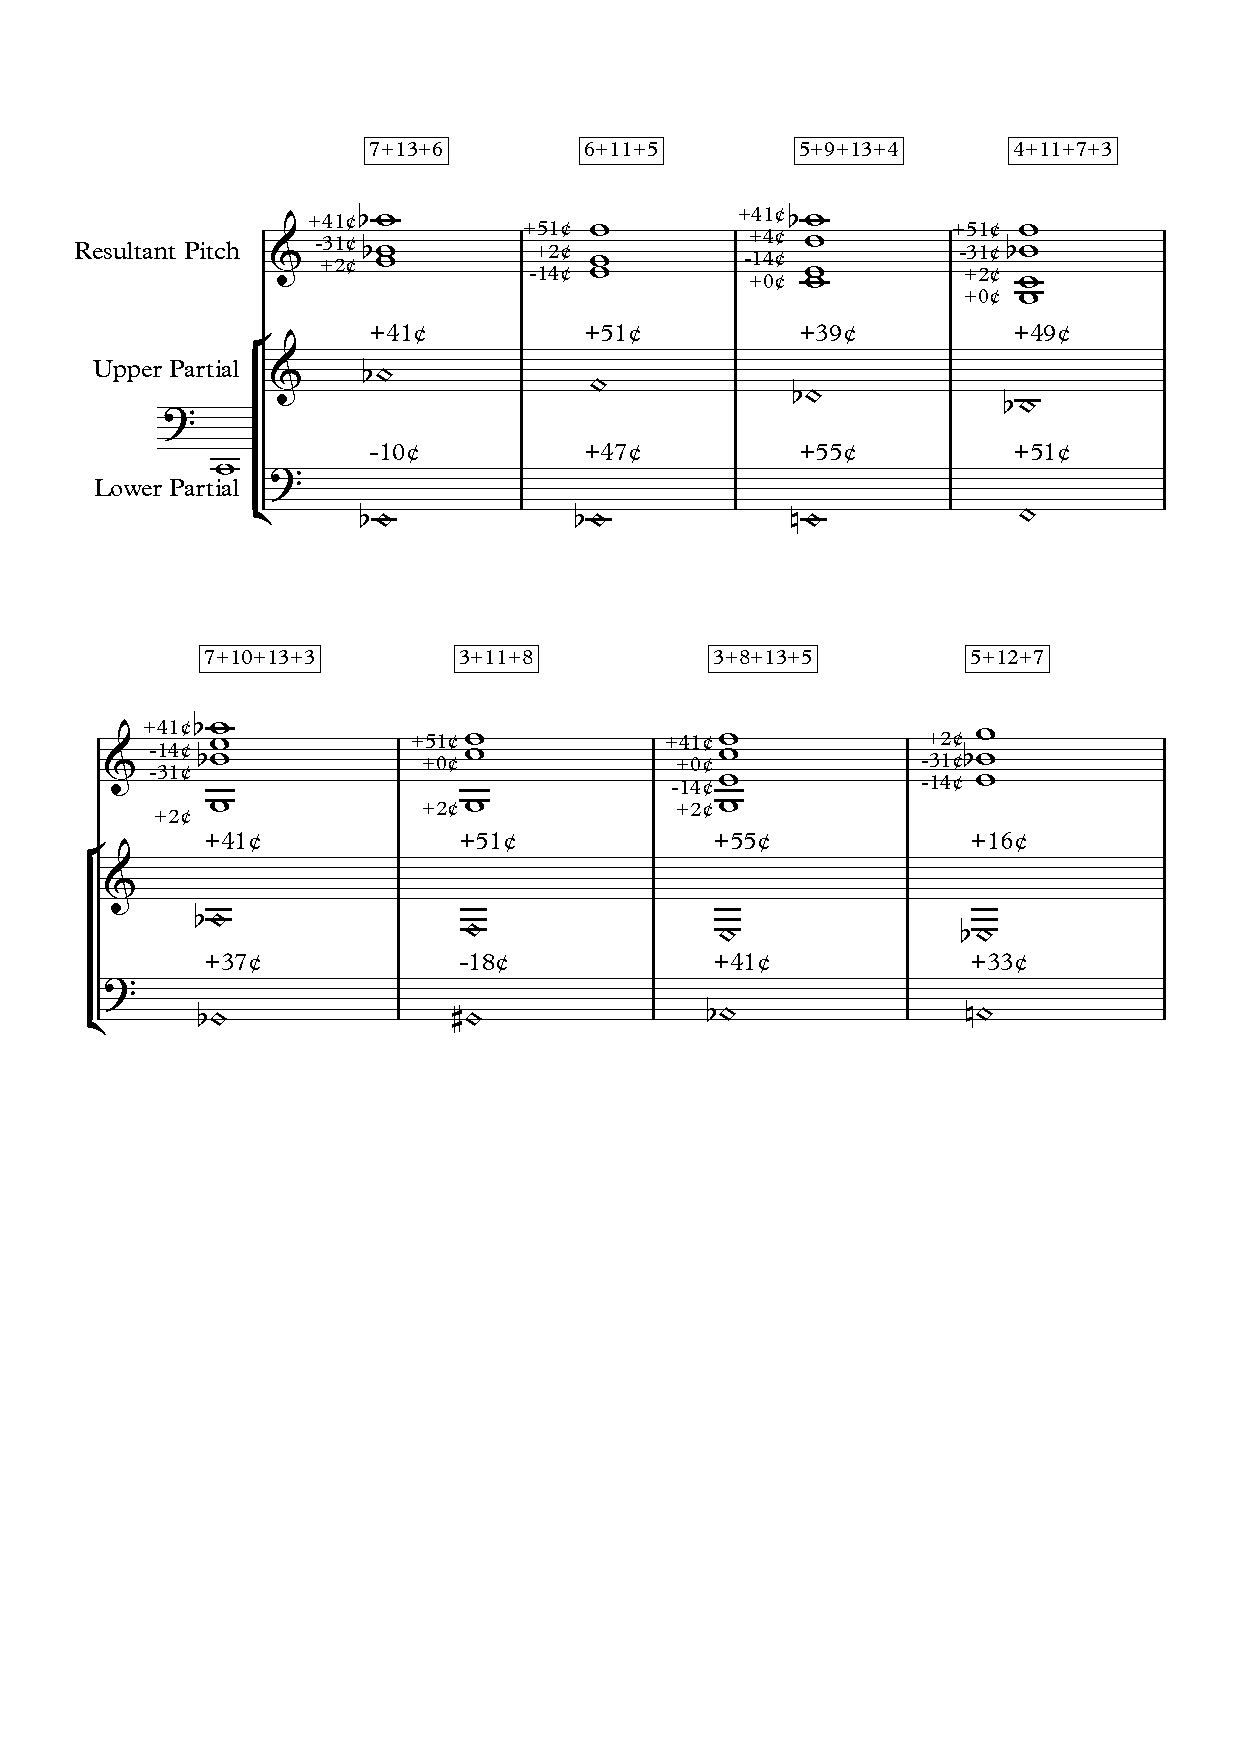
\includepdf[pages=-,pagecommand={}]{resources/multiphonicFingeringChart.pdf}
    % app1.tex (file to switch to appendix mode)
\newpage

% \invisiblechapter{\violinPiece}
\chapter[\violinPiece]{}


\vspace*{3cm}
\begin{center}
\textsc{for solo violin}
\vspace*{3.5cm}

\HRule{0.5pt}


\LARGE \textbf{\uppercase{\violinPiece}}
\HRule{2pt}

\vspace{1.3cm}

\normalsize October, 2019
\date{}

\vspace*{5\baselineskip}

Rhys Gray

\end{center}
\newpage
\section*{Program Notes}
% \violinPiece\space is a solo work for violin that explores \hyperref[sec:half-harmonics]{half-harmonics}.
It is a non-programmatic work, and the title was inspired by a question that my supervisor posed to me while I sought ethics approval for my exegesis; a simple phrase laden with possible contexts, spurring the imagination to try and complete the meaning.

% It is, in a way, an etude, treating the half-harmonics in a way similar to those found in Sciarrino's \hyperref[fig:sciarrinoExcerpt]{\emph{6 Caprricio for violin}}. 
Half-harmonics are produced by applying left hand finger pressure halfway between that required to create a harmonic, and a \emph{normale} sound. 
The sound that is produced should be a mixture of the stopped string pitch, the harmonic pitch, and a resistant, slightly noisy quality.
% They are notated in the score as a half-filled diamond notehead.

\section*{Notation}
\begin{itemize}

    \item Half-harmonics are notated in the score as a half-filled diamond notehead.
    \item Arrows denote gradual transitions to the technique that the arrow is pointing to.\begin{itemize}
        \item Arrows between notes denote transitions between the types of notes (i.e.\ \emph{normale} to harmonic finger pressure.)
      \end{itemize}
    % \item sp denotes \emph{sul ponticello}.
    % \item msp denotes \emph{molto sul ponticello}.
    % \item similarly, st denotes \emph{sul tasto}, and mst denotes \emph{molto sul tasto}
\end{itemize}

\newpage\label{app:violinPiece Score}
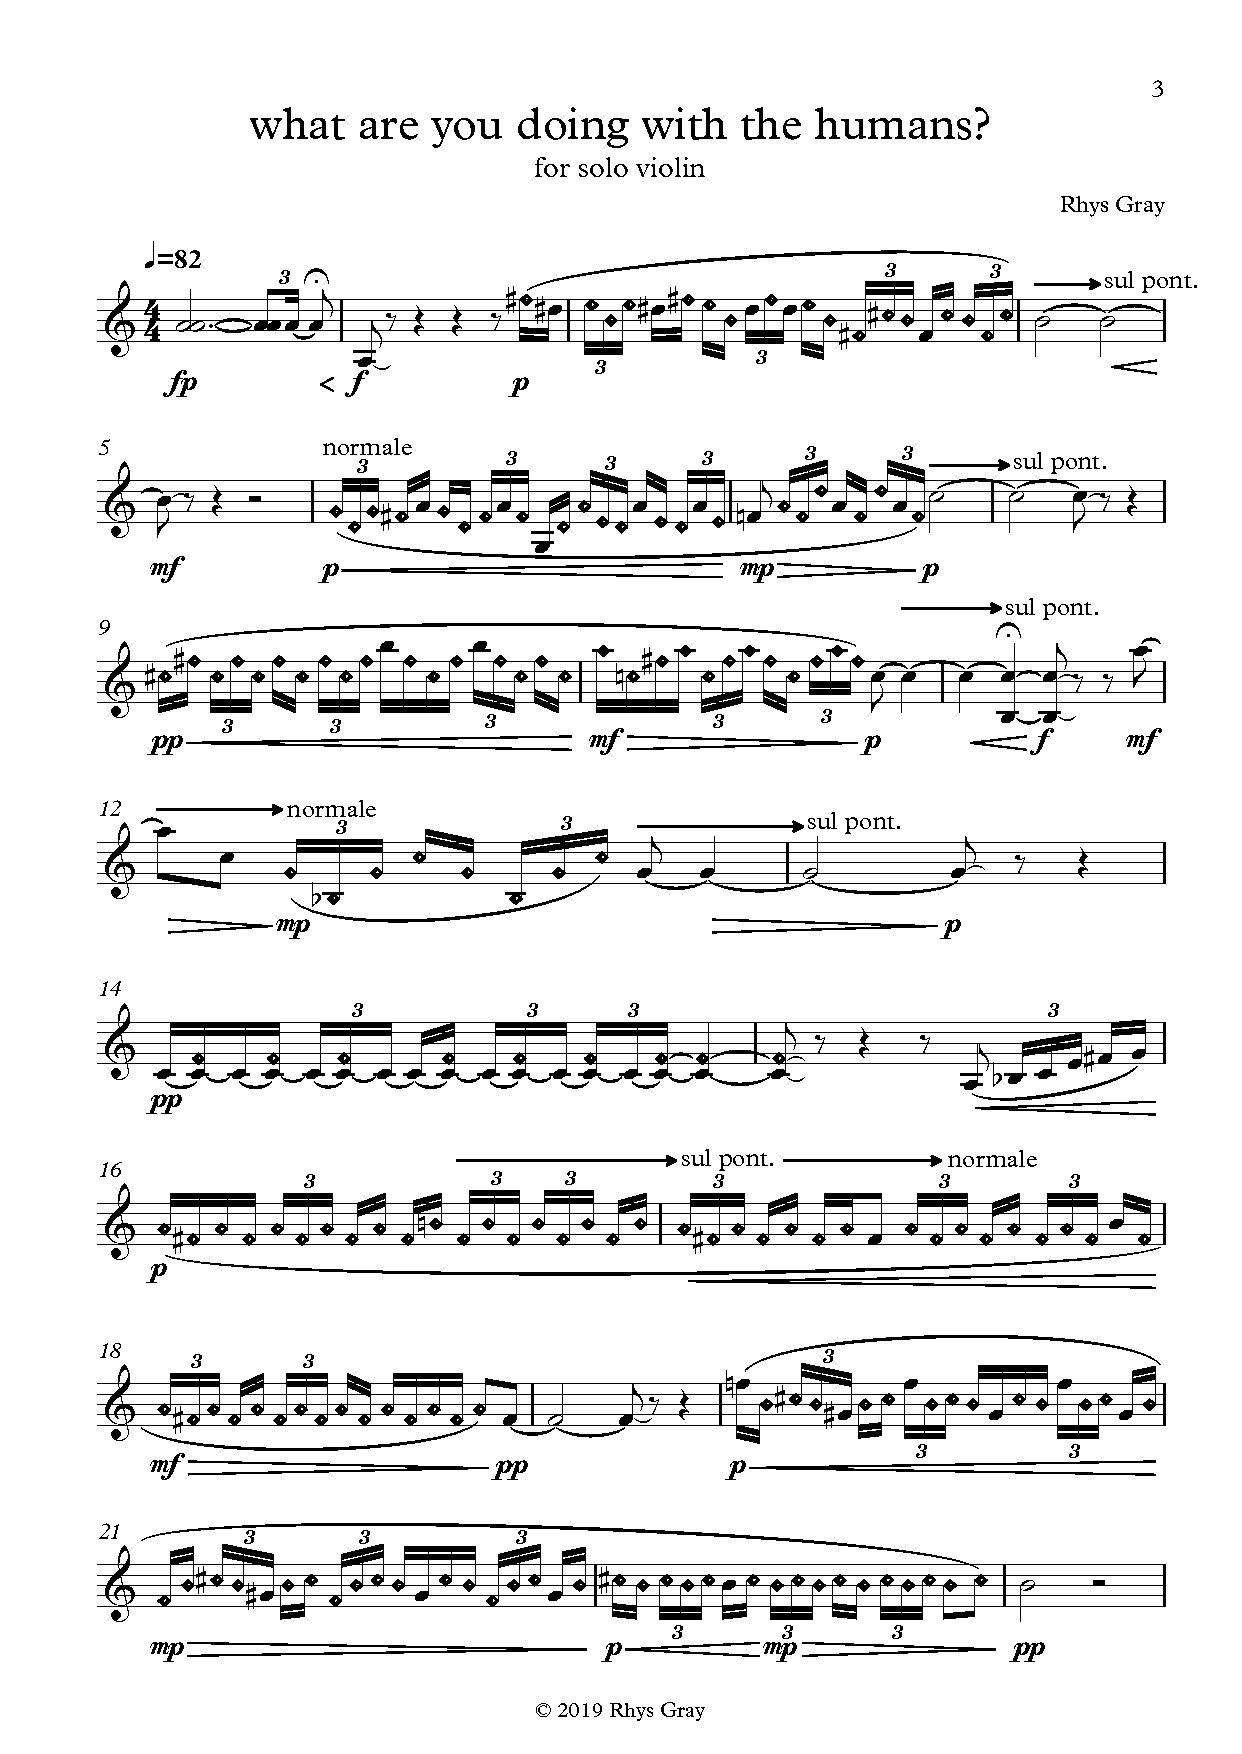
\includepdf[pages=-,pagecommand={}]{resources/compositions/violin.pdf}
    % % app2.tex (file to switch to appendix mode)

\chapter[\violaPiece]{}

\vspace*{3cm}
\begin{center}
\textsc{for solo viola}

\vspace*{3.5cm}

\HRule{0.5pt}


\LARGE \textbf{\uppercase{\violaPiece}}
\HRule{2pt}

\vspace{1.3cm}

\normalsize October, 2019
\date{}

\vspace*{5\baselineskip}

Rhys Gray

\end{center}
\newpage
\newpage

\section*{Program Notes}
\violaPiece\space is a piece for solo viola, written to explore the lower register of the viola using \hyperref[sec:subharmonics]{subharmonics} juxtaposed with upper harmonics. 

Subharmonics are achieved through precise control of torsional oscillation, which usually produces the sound of an amateur string player's heavy handed, slow bowing. 

To play subharmonics, one should place the bow at the 6th partial of the harmonic series of the fingered pitch, and bow with excessive pressure and an absolutely consistent speed. 
The increased pressure will distort the vibration of the string, producing a phase loop which, in turn, produces the subharmonic. 


The production of subharmonics can be aided by using older strings (which work better due to fats building up on the strings). 
Making a counter-clockwise half-twist in the string can also make it easier to produce octave and major second subharmonics (additional twists can help achieve lower subharmonics, at the expense of higher ones).

\section*{Notation}
\begin{itemize}

    \item Subharmonics are notated in the score using a square notehead for the fingering, with a small notehead at the desired resultant pitch. Where additional clarification is needed, `sh' is placed above.
    \item Arrows denote gradual transitions to the technique that the arrow is pointing to.\begin{itemize}
        \item Arrows between notes denote transitions between the types of notes (i.e.\ \emph{normale} to harmonic finger pressure.)
      \end{itemize}
    \item sp denotes \emph{sul ponticello}.
    \item msp denotes \emph{molto sul ponticello}.
    \item similarly, st denotes \emph{sul tasto}.
    \item n denotes \emph{normale}.
    \item Feathered beams denote a gradual acceleration to a tremolo.
\end{itemize}

\newpage\label{app:violaPiece Score}

% 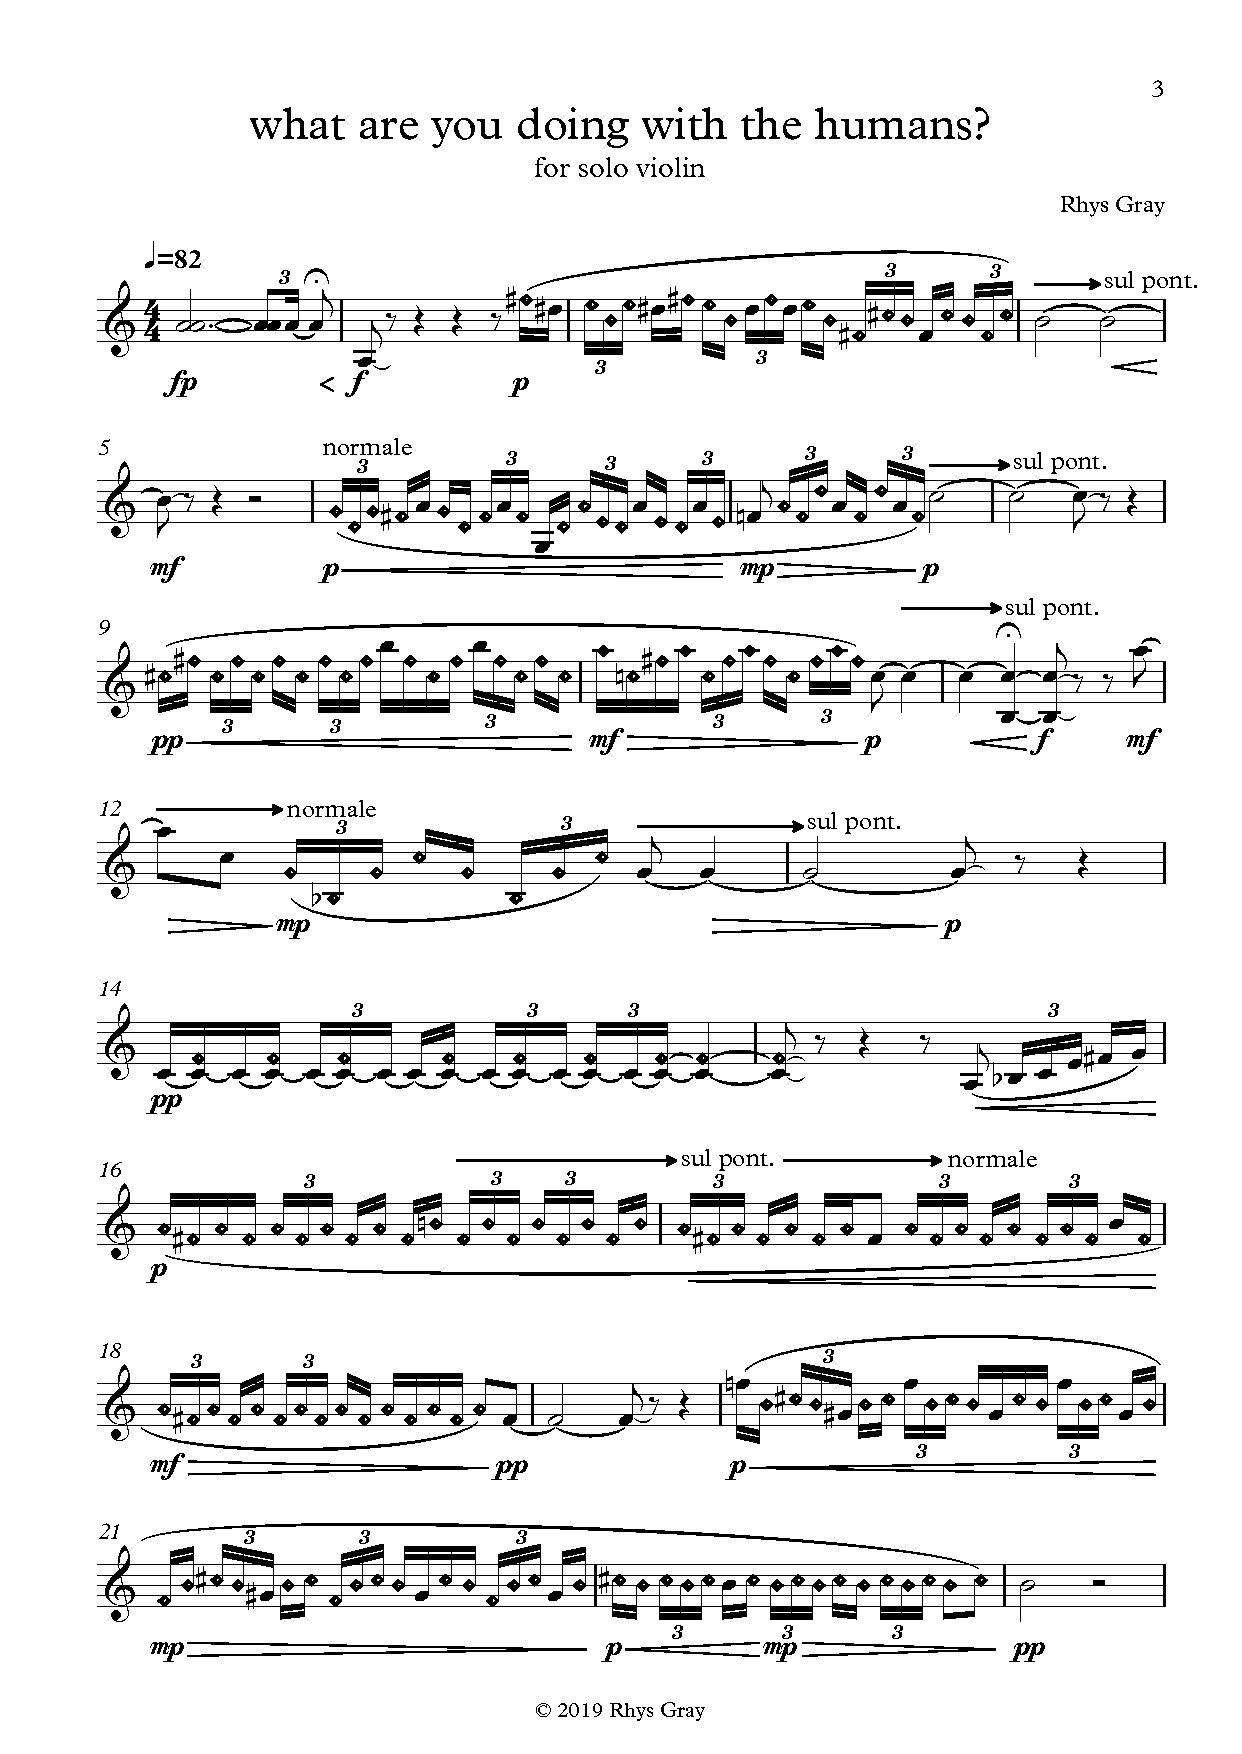
\includepdf[pages=-,pagecommand={},width=\textwidth]{resources/compositions/violin.pdf}
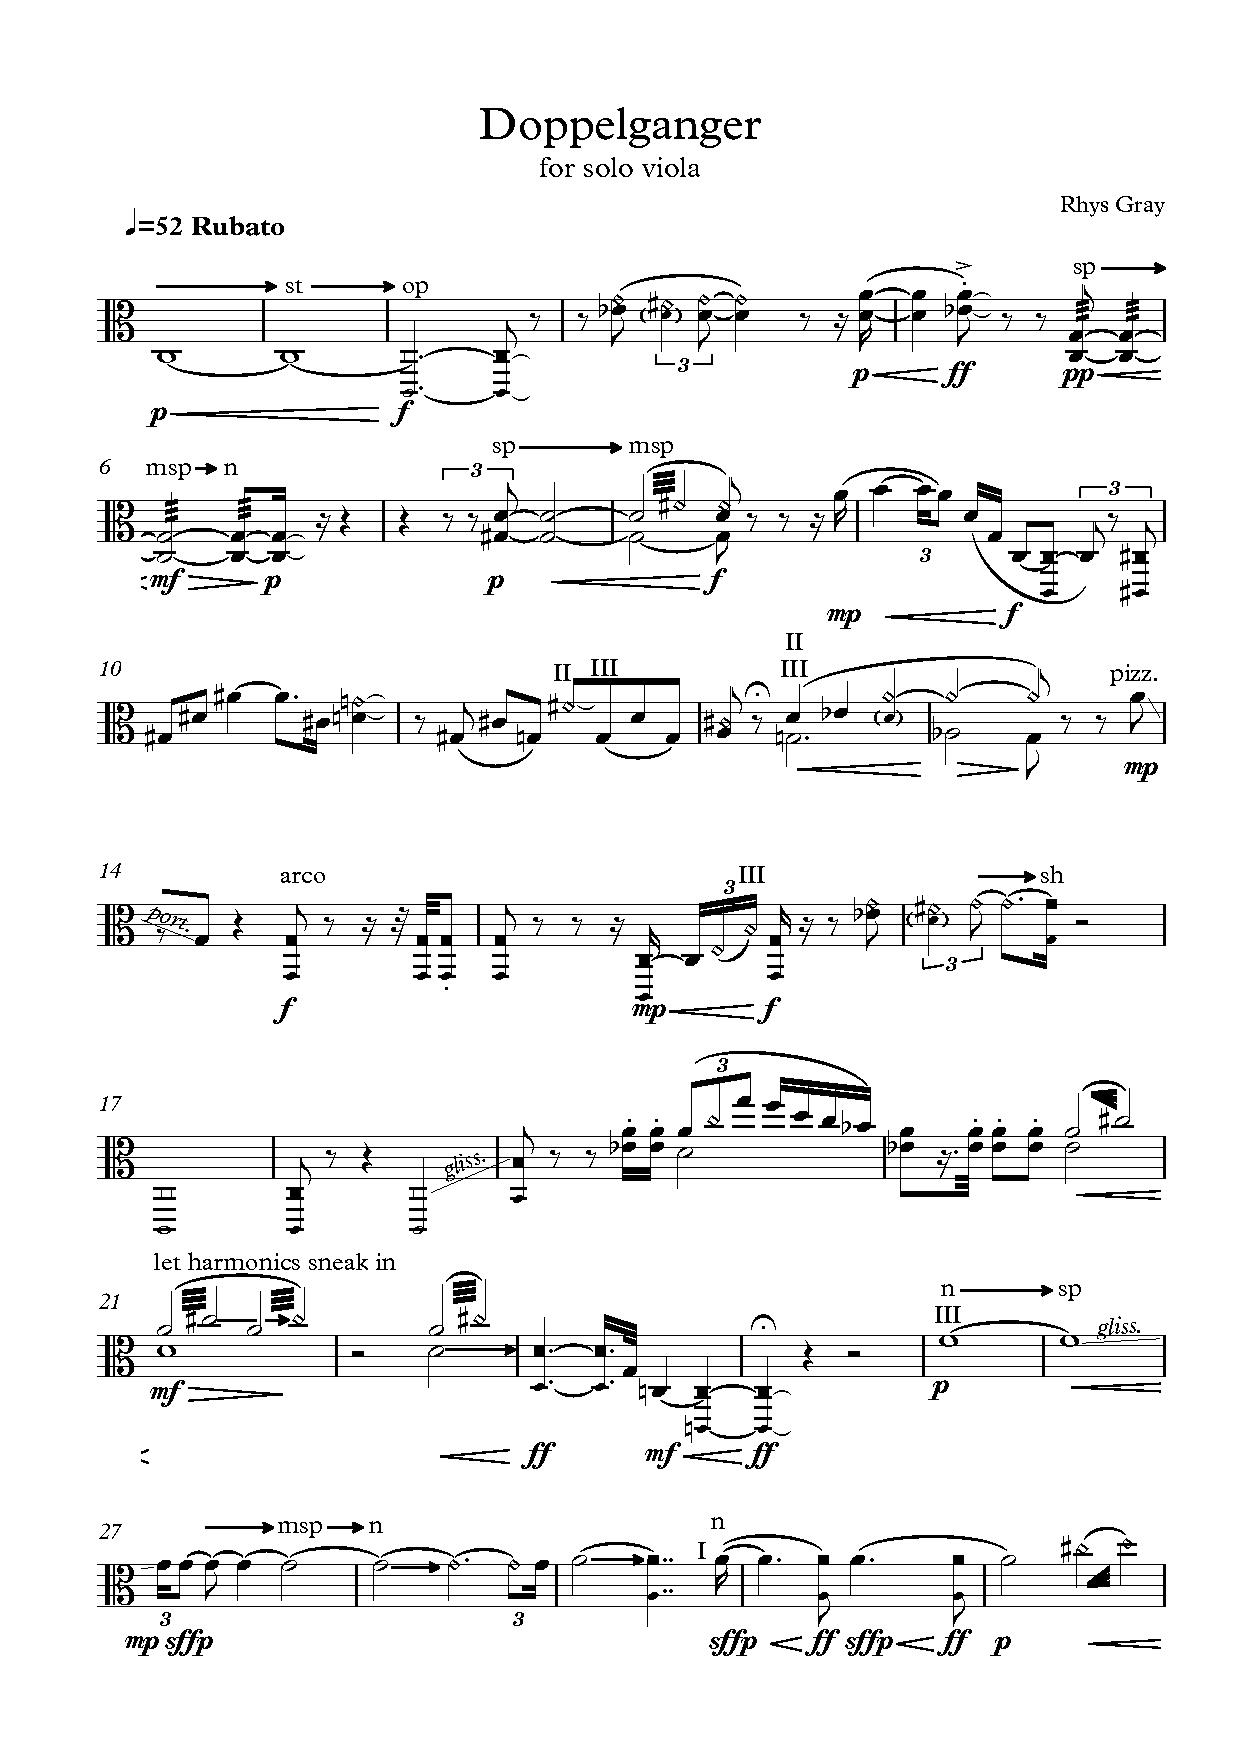
\includepdf[pages=-,pagecommand={}]{resources/compositions/viola.pdf}
    % % app2.tex (file to switch to appendix mode)

\chapter[\celloPiece]{}

\vspace*{3cm}
\begin{center}
\textsc{for solo violoncello}

\vspace*{3.5cm}

\HRule{0.5pt}


\LARGE \textbf{\uppercase{\celloPiece}}
\HRule{2pt}

\vspace{1.3cm}

\normalsize October, 2019
\date{}

\vspace*{5\baselineskip}

Rhys Gray

\end{center}
\newpage
\newpage

\section*{Program Notes}
\celloPiece\space is a piece for solo violoncello, written to explore \hyperref[sec:multiphonics]{multiphonics}. 

Multiphonics are achieved through clusters of close harmonic nodes, and by playing a harmonic close to the highest partial.
  Note that not all of these pitches will actually sound in practice.
  
  Multiphonics are notated as a harmonic position using a diamond notehead, with an `M' above the note to be fingered.
  Where the string used is ambiguous, it is notated below the sounding pitch as a small, bracketed notehead.
  Precise tuning is given in cents, and unless otherwise notated, is intended for the first note that the multiphonic is attached to.\footnote{100 cents is equal to a semitone. Therefore, +51c is roughly equal to half a semitone sharp. Cents have been used due to their precision compared to more granular accidentals such as the quartertone sharp.}
  The theoretical sounding pitches are given in a bracketed staff above the main stave.
  % Above the sounding pitches, the sounding partials are given (i.e. M IV [4th + 13th + 9th + 15th + 5th]).

  The bow should exert slightly more pressure than usual and should be drawn with a consistent speed which should be slower than for harmonics.
  The location of the bow can encourage or discourage upper or lower partials, and experimentation should be done during the practice of this work to achieve the pitches desired.

\section*{Notation}
\begin{itemize}
  \item Multiphonics are denoted with a diamond notehead, marked with an M (see \autoref{fig:multiphonicsBassExample} for an example). 
  \begin{itemize}
    \item Precise tuning in cents (i.e. +41c) is provided to help the performer pitch the fingering required for the multiphonic to be produced.
    \item The multiphonic resultant pitches are notated at pitch in the \emph{suono reale} stave, with the cents tuning of the resultant pitches to the left or right of the notes.
  \end{itemize}
    \item Arrows denote gradual transitions to the technique that the arrow is pointing to.\begin{itemize}
      \item Arrows between notes denote transitions between the types of notes (i.e.\ \emph{normale} to harmonic finger pressure.)
    \end{itemize}
    \item n denotes \emph{normale}.
    % \item sp denotes \emph{sul ponticello}.
    % \item msp denotes \emph{molto sul ponticello}.
    % \item similarly, st denotes \emph{sul tasto}, and mst denotes \emph{molto sul tasto}
\end{itemize}

\newpage\label{app:celloPiece Score}
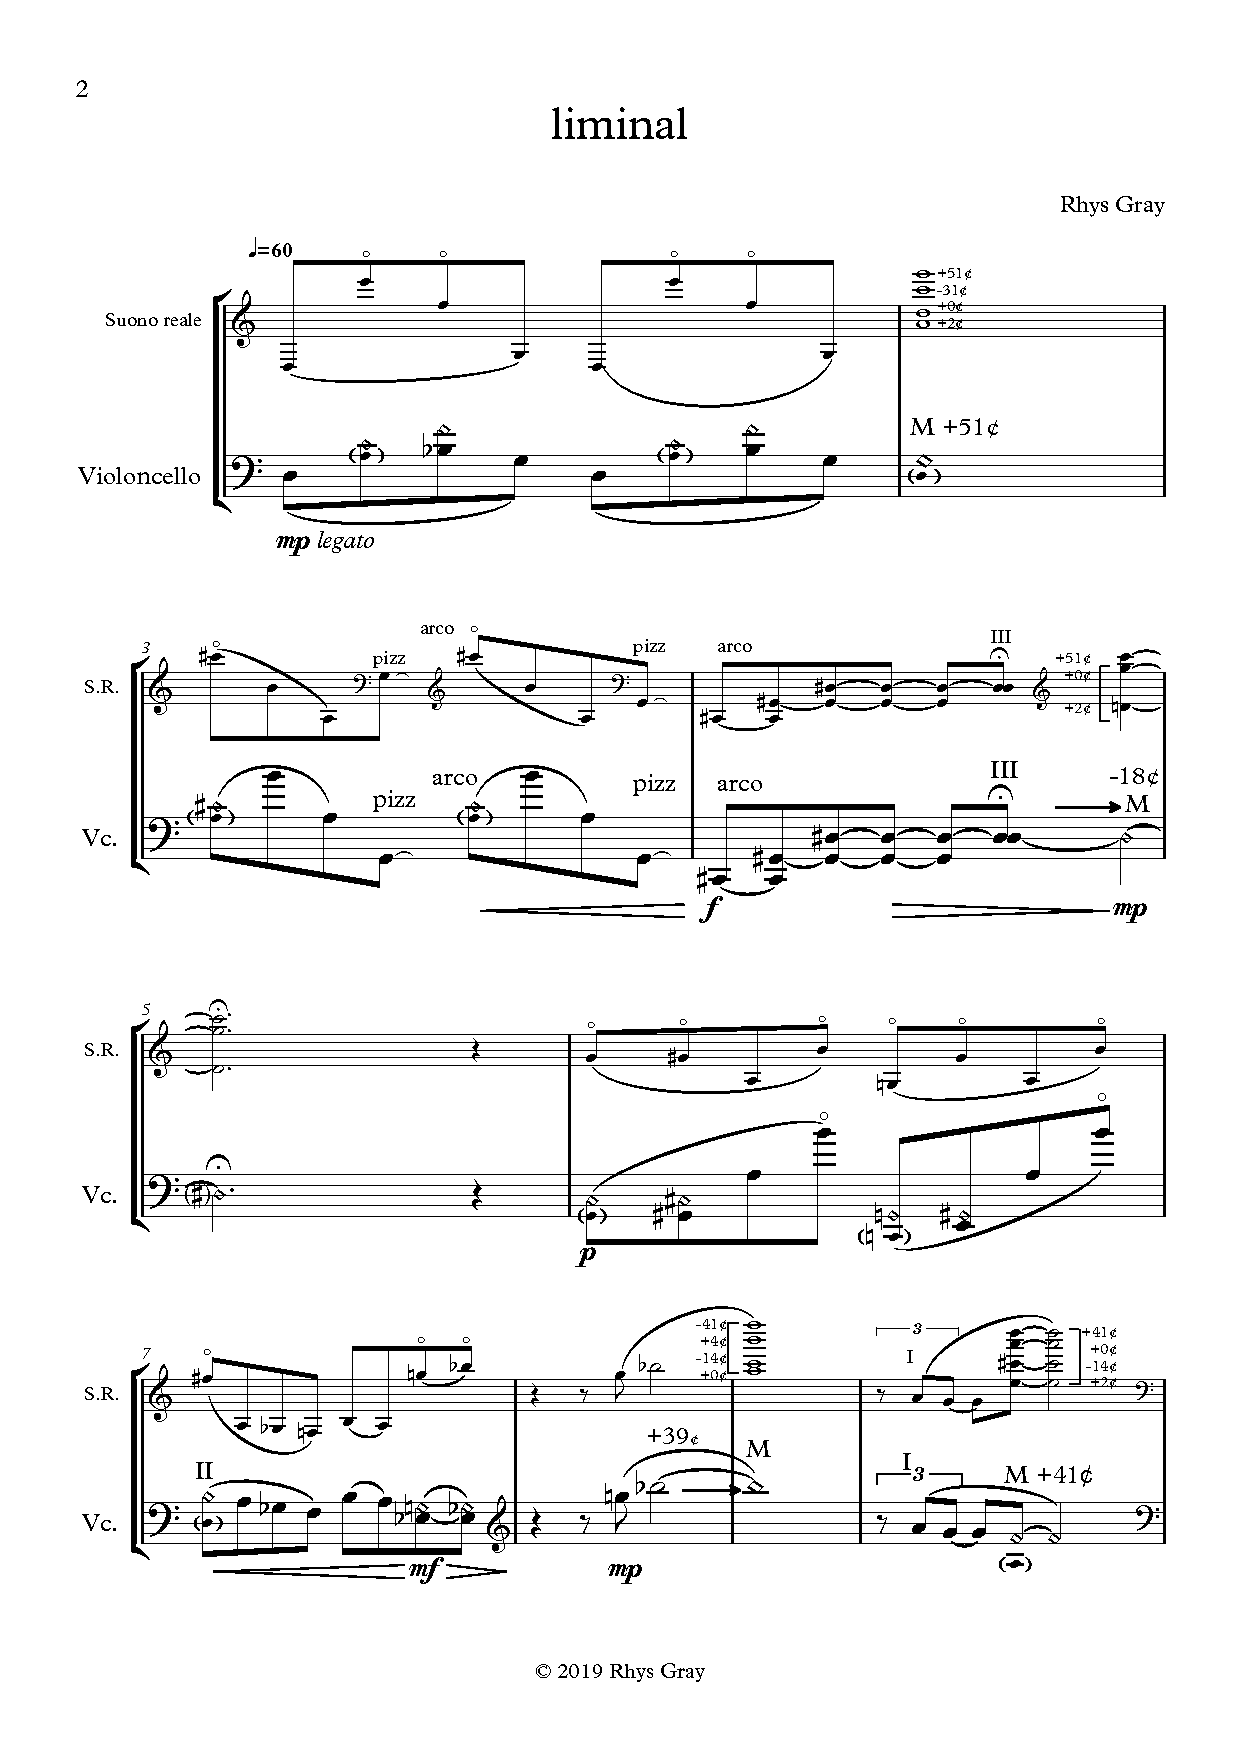
\includepdf[pages=-,pagecommand={}]{resources/compositions/violoncello.pdf}
    % % app2.tex (file to switch to appendix mode)

\chapter[\bassPiece]{}

\vspace*{3cm}
\begin{center}
\textsc{for solo contrabass}

\vspace*{3.5cm}

\HRule{0.5pt}


\LARGE \textbf{\uppercase{\bassPiece}}
\HRule{2pt}

\vspace{1.3cm}

\normalsize October, 2019
\date{}

\vspace*{5\baselineskip}

Rhys Gray

\end{center}
\newpage
\newpage

\section*{Program Notes}
Inspired by the eponymous short story by Ray Bradbury, \bassPiece\space is a composition for solo contrabass, and uses \hyperref[sec:subharmonics]{subharmonics} and \hyperref[sec:multiphonics]{multiphonics}. 
Similarly like the namesake, this world is filled with danger but also beauty. 
It is non-programmatic, and my intent with Veldt was to create a soundworld and space that the performer was able to `roam around' in, and features several sections of improvisation on pitch-sets.

\subsubsection*{Subharmonics}
Subharmonics are achieved through precise control of torsional oscillation, which usually produces the sound of an amateur string player's heavy handed, slow bowing. 

To play subharmonics, one should place the bow at the 6th partial of the harmonic series of the fingered pitch, and bow with excessive pressure and an absolutely consistent speed. 
The increased pressure will distort the vibration of the string, producing a phase loop which, in turn, produces the subharmonic. 
The production of subharmonics can be aided by using older strings (which work better due to fats building up on the strings). 
Making a counter-clockwise half-twist in the string can also make it easier to produce octave and major second subharmonics (additional twists can help achieve lower subharmonics, at the expense of higher ones).

\subsubsection*{Multiphonics}
Multiphonics are achieved through clusters of close harmonic nodes, and by playing a harmonic close to the highest partial.
  Note that not all of these pitches will actually sound in practice.
  
  Multiphonics are notated as a harmonic position using a diamond notehead, with an `M' above the note to be fingered.
  Where the string used is ambiguous, it is notated below the sounding pitch as a small, bracketed notehead.
  Precise tuning is given in cents, and unless otherwise notated, is intended for the first note that the multiphonic is attached to.\footnote{100 cents is equal to a semitone. Therefore, +51c is roughly equal to half a semitone sharp. Cents have been used due to their precision compared to more granular accidentals such as the quartertone sharp.}
  The theoretical sounding pitches are given in a bracketed staff above the main stave.
  % Above the sounding pitches, the sounding partials are given (i.e. M IV [4th + 13th + 9th + 15th + 5th]).

  The bow should exert slightly more pressure than usual and should be drawn with a consistent speed which should be slower than for harmonics.
  The location of the bow can encourage or discourage upper or lower partials, and experimentation should be done during the practice of this work to achieve the pitches desired.

\section*{Notation}
\begin{itemize}

    \item Subharmonics are notated in the score using a square notehead for the fingering, with a small notehead at the desired resultant pitch. Where additional clarification is needed, `sh' is placed above.
    \begin{itemize}
      \item They are notated at pitch in the cue sized stave above, with a harmonic circle above them.
    \end{itemize}
    \item Multiphonics are denoted with a diamond notehead, marked with an M (see \autoref{fig:multiphonicsBassExample} for an example). 
    \begin{itemize}
      \item Precise tuning in cents (i.e. +41c) is provided to help the performer pitch the fingering required for the multiphonic to be produced.
      \item The multiphonic resultant pitches are notated at pitch in the cue sized stave above, with the cents tuning of the resultant pitches to the left or right of the notes.
    \end{itemize}
    \item Arrows denote gradual transitions to the technique that the arrow is pointing to.\begin{itemize}
      \item Arrows between notes denote transitions between the types of notes (i.e.\ \emph{normale} to harmonic finger pressure.)
    \end{itemize}
    \item Sounding pitch is provided in the ossia stave above.
    \item Bridge position is provided in the stave above, and denotes the vertical location of the bow. The bottom line is \emph{molto sul tasto} and the top line is \emph{molto sul ponticello}.
    \item For un-metered bars, approximate times are given above in seconds, and is linearly proportional (i.e.\ note spacing denotes approximate time.)
    \item Repeats are to be repeated for as long as instructed.
    % \item \emph{battuto} is letting the bow hit the string, with no horizontal movement.
    % \item \emph{gettato} is like battuto, but with a slight amount of horizontal movement.
    % \item \emph{jeté} is bouncing the bow on the string, letting gravity do the work in conjunction with horizontal movement.
    \item op denotes overpressure.
    \item sp denotes \emph{sul ponticello}.
    \item n denotes \emph{normale}.
    % \item msp denotes \emph{molto sul ponticello}.
    % \item similarly, st denotes \emph{sul tasto}, and mst denotes \emph{molto sul tasto}
\end{itemize}

\newpage\label{app:bassPiece Score}

% 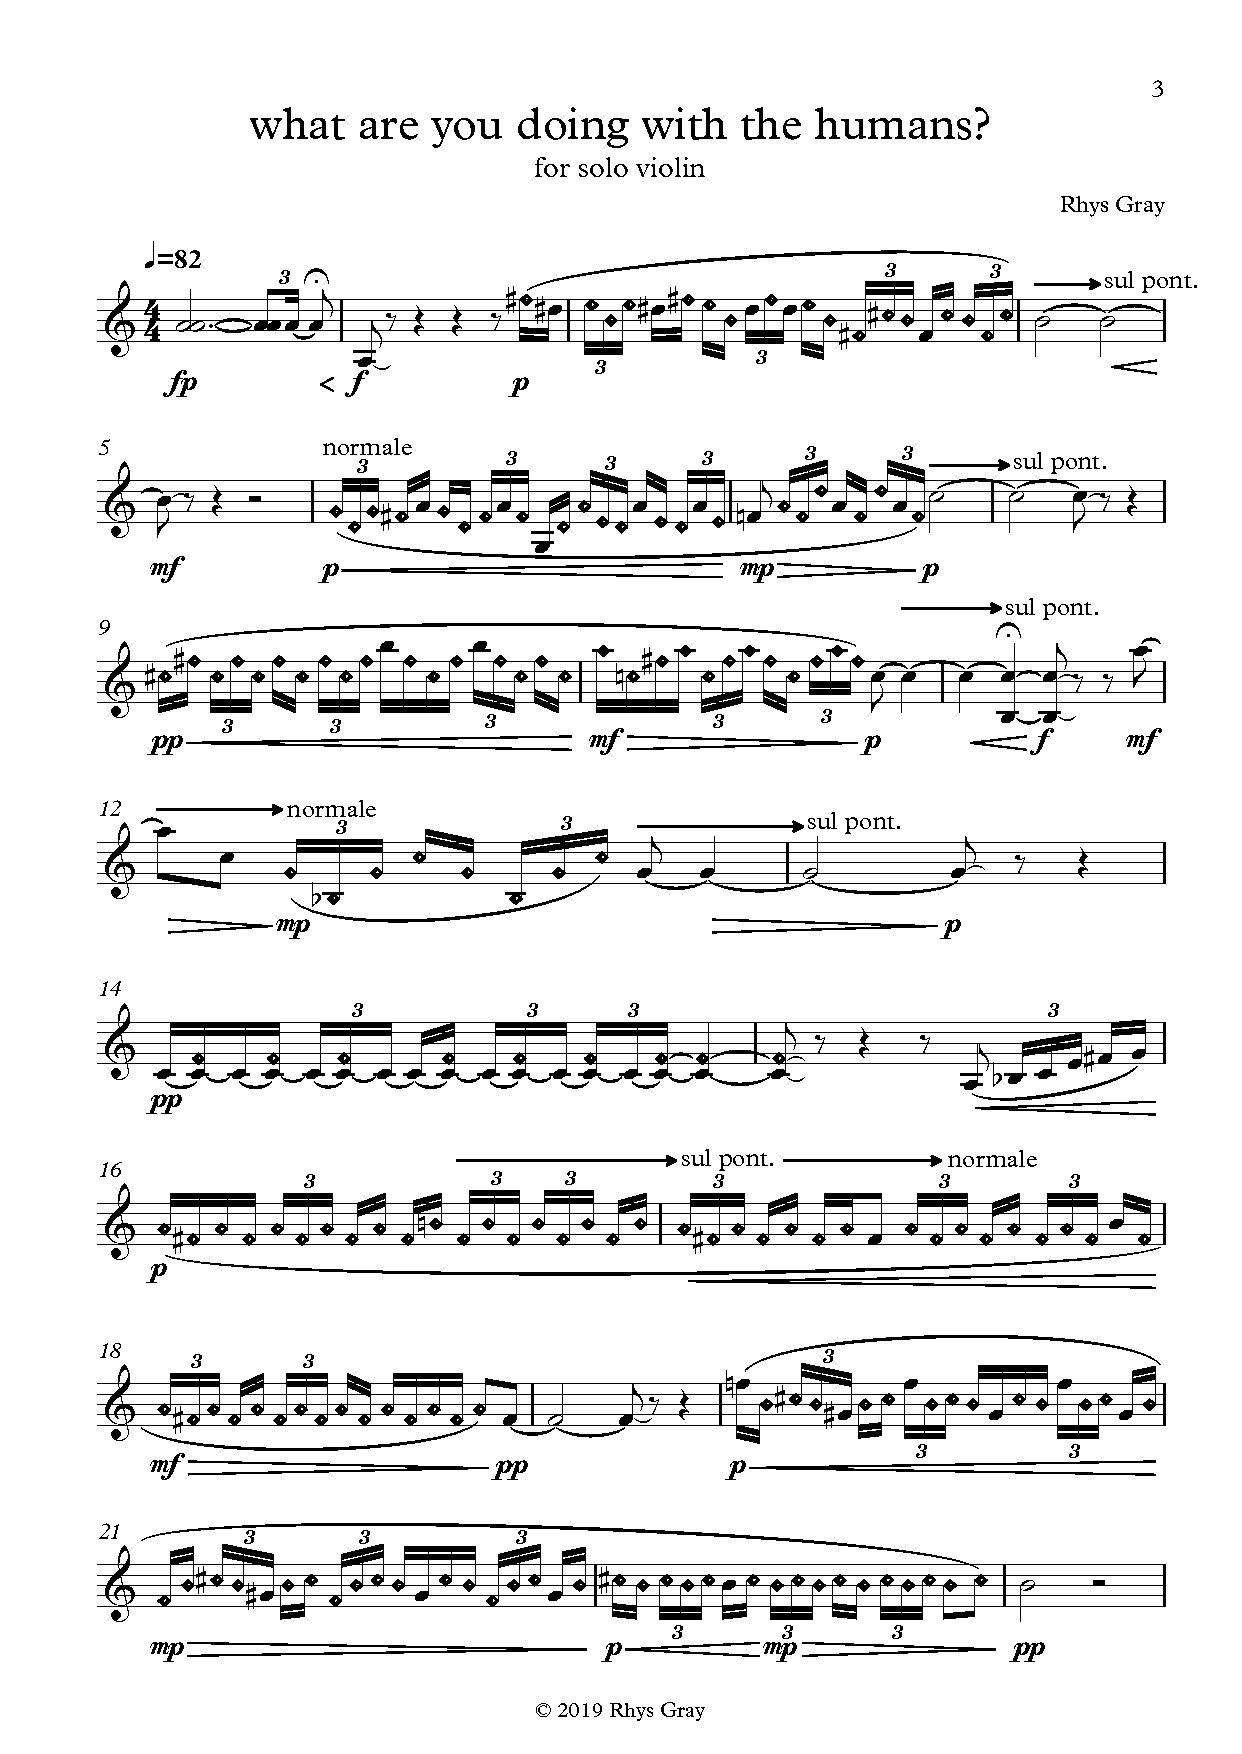
\includepdf[pages=-,pagecommand={},width=\textwidth]{resources/compositions/violin.pdf}

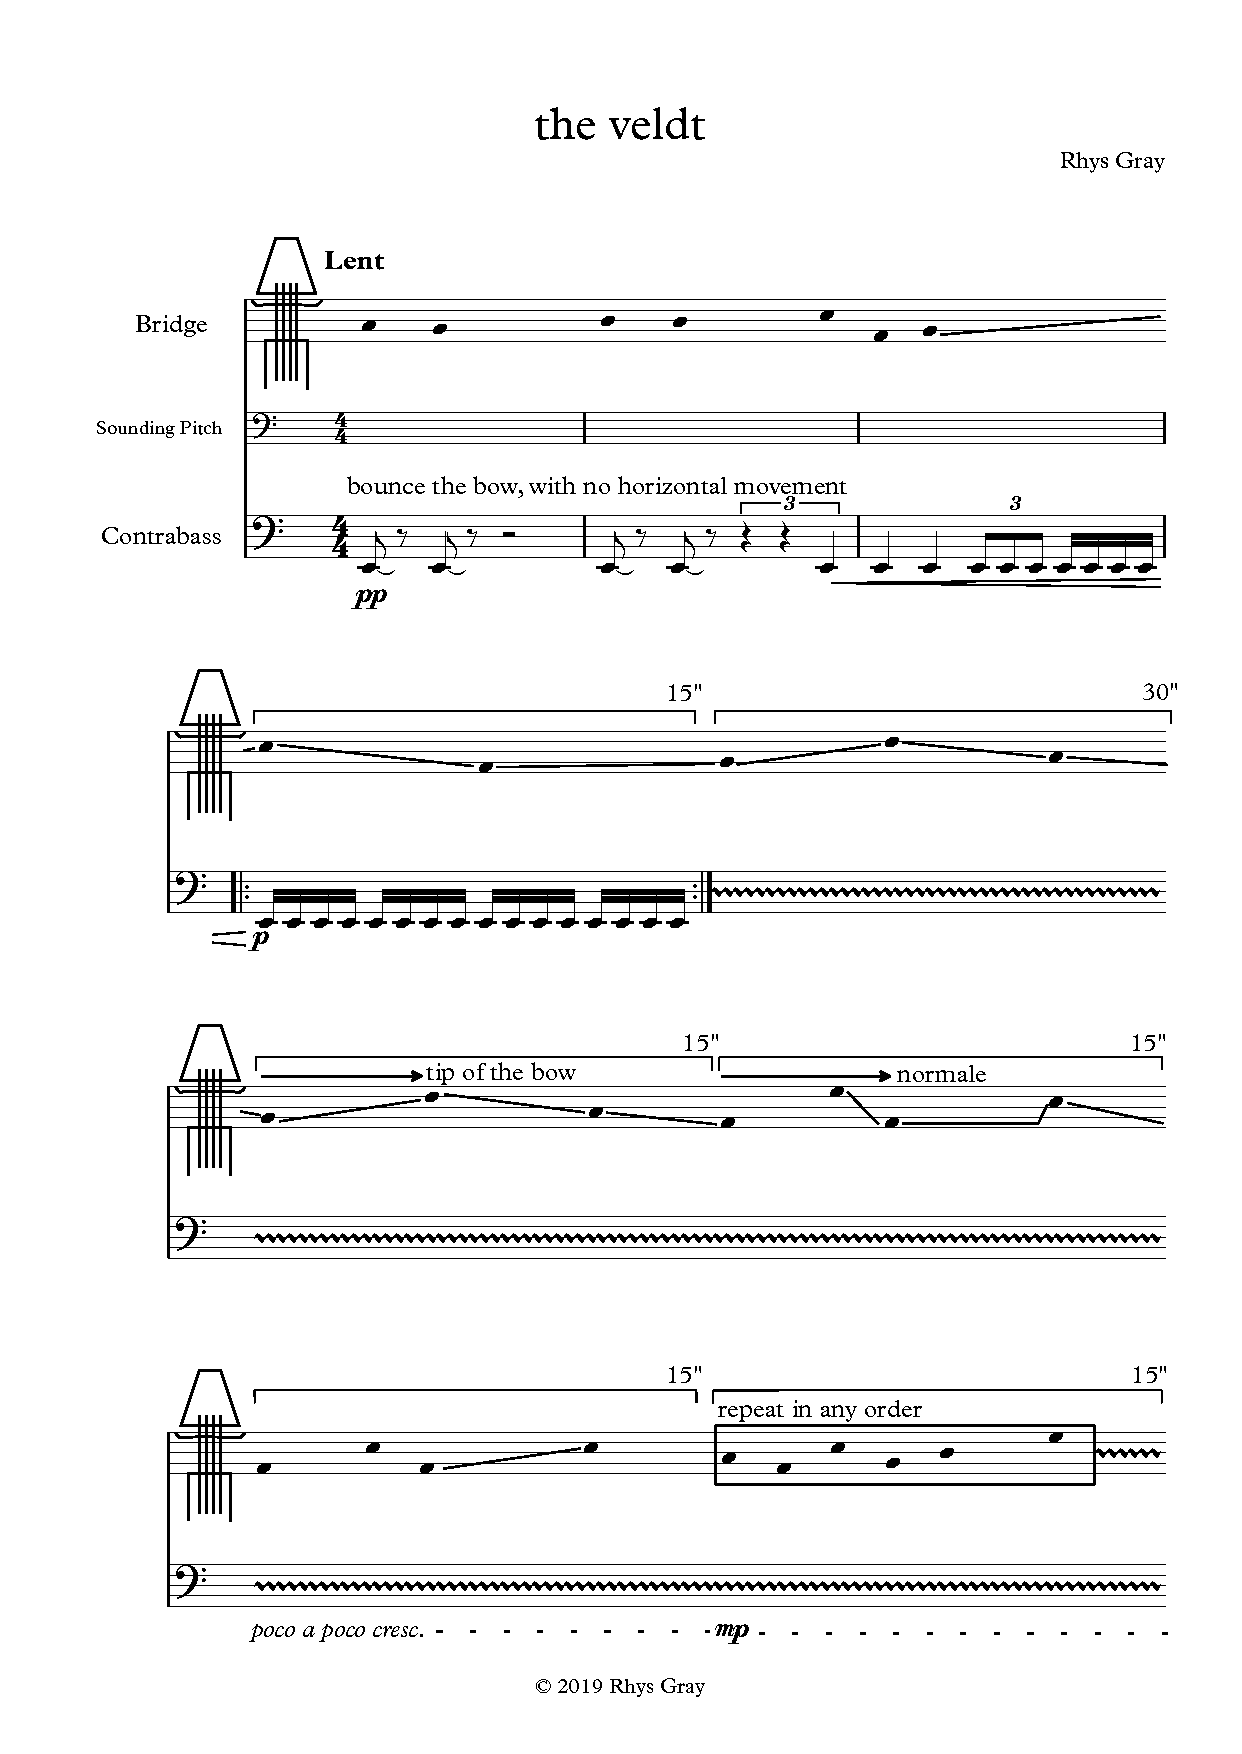
\includepdf[pages=-,pagecommand={}]{resources/compositions/bass.pdf}
    % \include{backmatter/appendixb}
\end{appendixes}

\printbibliography{}

\end{document}
